\documentclass{article}

\usepackage[margin=1in]{geometry}
\usepackage{graphicx}
\usepackage{amsmath}
\usepackage{caption}
% \captionsetup[table]{skip=5pt}  % table caption too close
\usepackage{booktabs} % better tables
\usepackage{subfig}
\usepackage{algpseudocode}
\usepackage{algorithm}
\usepackage[colorlinks,bookmarks,bookmarksnumbered,allcolors=blue]{hyperref}
\usepackage[capitalise]{cleveref}


\begin{document}

\author{Andrew Ning}
\title{A More Thorough Development of\\Blade Element Momentum Theory}
\date{March 7, 2017}
\maketitle
% :\\Considering All Inflow Angles, Turbines and Propellers, and Yawed Inflow

\section{Introduction}

The basic blade element momentum theory works well for on-design operation and is detailed in many references.  For the standard case, the author has developed a reformulated approach that simplifies the solution processes and is provably convergent \cite{Ning2014-Simple-Solution}.  However, when considering operation under turbulent conditions, gusts, maneuvers, with flexible blades, and in other non-ideal operating scenarios, a more complete derivation is needed.  In this derivation we extend basic blade element momentum theory to consider all possible inflow angles, large axial inductions, turbines and propellers simultaneously, and yawed inflow.

\section{Linear Momentum Balance}

We begin simply by applying mass and momentum balances for a streamtube passing through a rotor.  Rather than using one streamtube for the entire rotor disk, we use an annulus streamtube passing through a specific location of $r$ along the rotor (\cref{fig:annulus}). This will be more convenient when relating to blade element theory later.  Through most of the document we will use the conventions for wind turbines, but the theory is equally applicable to propellers/fans as well.  The small modifications necessary for propellers are discussed throughout.  We will use the term propellers to generically refer to any turbomachine that adds momentum to the fluid.

\begin{figure}[htbp]
\centering
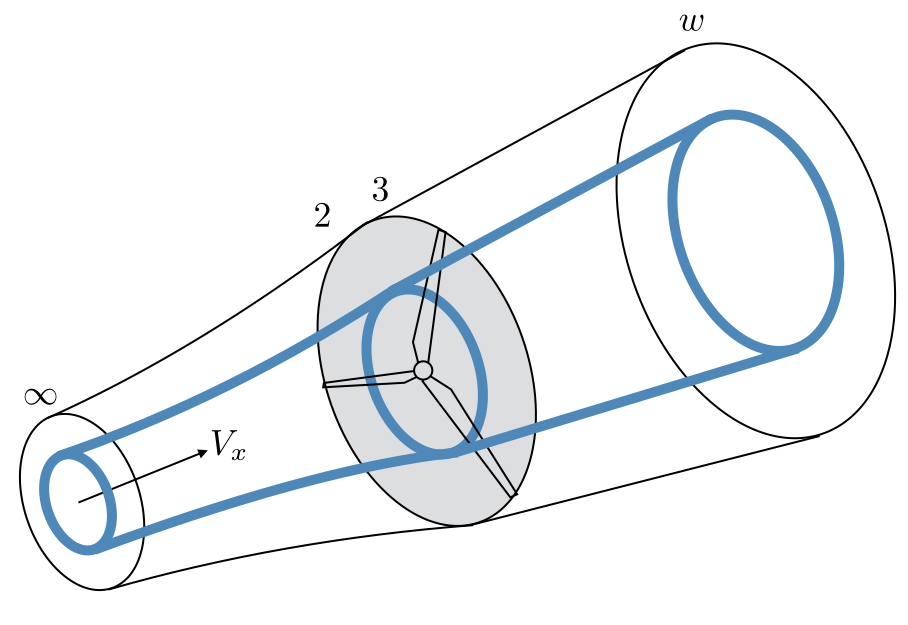
\includegraphics[width=3.25in]{figures/annulus}
\caption{The blue annulus streamtube is used as our control volume in the derivation of this section.  The stations are denoted by $\infty$: far upstream, $2$: just upstream of the disk, $3$ just downstream of the disk, and $w$ in the far wake.}
\label{fig:annulus}
\end{figure}

First, let's perform a mass balance.  In the following derivation we neglect any variations in density.  For a wind turbines an incompressibility assumption is reasonable, but for high-speed propellers some compressibility corrections may be necessary.  For the velocity upstream we will use $V_x$ rather than $V_\infty$ to match the convention used later in blade element theory.
\begin{equation}
    \rho V_x A_\infty = \rho V_2 A_2 = \rho V_w A_w
\end{equation}
Next, we apply an x-momentum balance across the entire control volume, where we take the positive direction for x as downwind:
\begin{equation}
    -\rho V_x^2 A_\infty + \rho V_w^2 A_w = - T
\end{equation}
We make no assumption about the direction of the thrust, but just use our sign convention for positive in the downwind direction and let the equations determine the direction of thrust (note that this is actually a drag force, but we use the conventions of wind turbines that call this a thrust force).  The minus sign occurs because a positive force implies that the force of the fluid on the turbine is downwind, hence the force of the turbine on the fluid is upwind.  Combining these two expressions yields:
\begin{equation}
\begin{aligned}
    T &= \rho A_2 V_2 (V_x - V_w)\\
    % &= \rho_2 A_d V_d (V_1 - V_4)
\end{aligned}
\label{eq:thrust1}
\end{equation}
% where $A_d$ is the rotor disk area and $V_d$ is the velocity at the rotor disk ($A_2 = A_3 = A_d$, and $V_2 = V_3 = V_d$).

It is not obvious that the pressure terms from the sides of our control volume cancel, but they do.  We can come up with the same result more rigorously, with the below control volume in \cref{fig:turbine-cv}.  Those details are omitted here, but can be found in \cite{?}.

\begin{figure}[htbp]
\centering
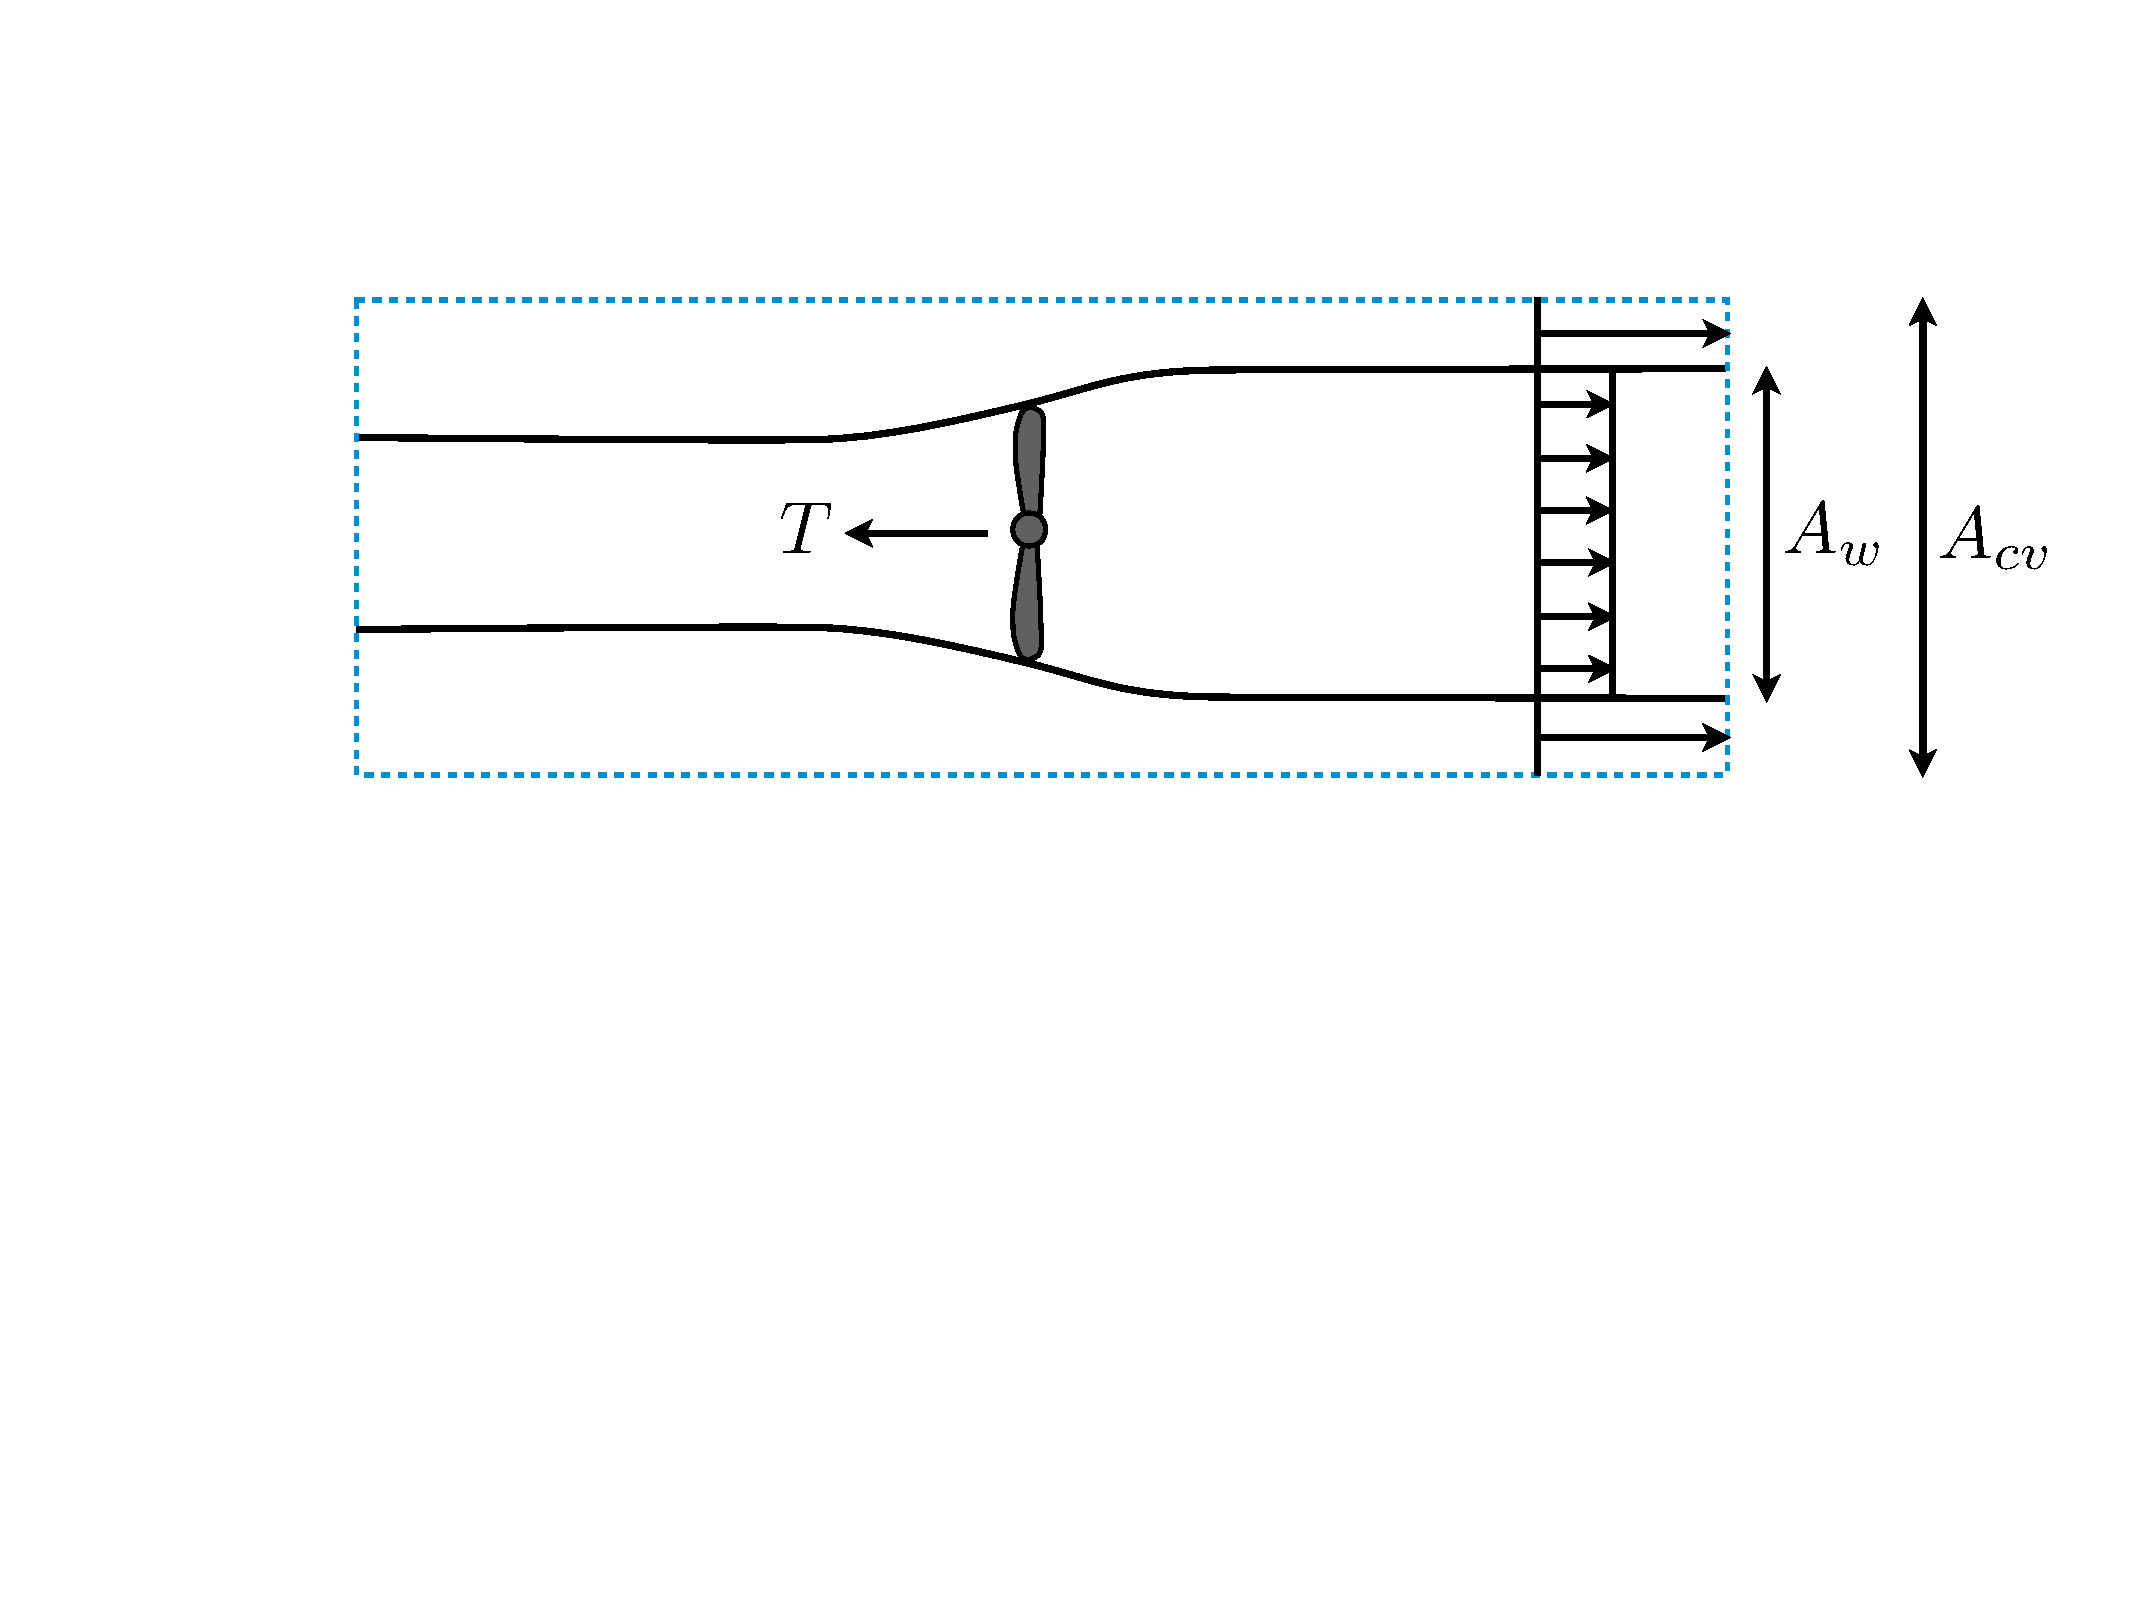
\includegraphics[width=3.5in]{figures/turbine-cv}
\caption{c}
\label{fig:turbine-cv}
\end{figure}

Let's now use a second control volume just across the disk (2 to 3).  Performing a momentum balance yields (neglecting any density changes across the disk):
\begin{equation}
\begin{aligned}
    0 &= - T + P_2 A_2 - P_3 A_3\\
    \Rightarrow T &= A_2 (P_2 - P_3)
\end{aligned}
\label{eq:thrust2}
\end{equation}
since $A_2 = A_3$.

Combining the two expressions for thrust yields (\cref{eq:thrust1,eq:thrust2}):
\begin{equation}
    \rho V_2 (V_x - V_w) = (P_2 - P_3)
    \label{eq:momentum1}
\end{equation}

To relate the pressure change from station 2 to 3, we will use Bernoulli's equation.  The assumptions for the form of Bernoulli's equation we use are that the flow must be inviscid and incompressible, there must not be any work done on the fluid, there must not be any heat transfer, and it is only applicable along a streamline.  Other versions of Bernoulli's equation exist where we can relax some of these assumptions, for our purposes they are reasonable assumptions upstream of the turbine and downstream of the turbine separately.  Note, we cannot apply Bernoulli's equation from station 2 to station 3 directly because work is done on the fluid.

First, from station $\infty$ to station 2:
\begin{equation}
    P_\infty + \frac{1}{2}\rho V_x^2 = P_2 + \frac{1}{2}\rho V_2^2
\end{equation}
then from station 3 to station $w$:
\begin{equation}
    P_3 + \frac{1}{2}\rho V_3^2 = P_w + \frac{1}{2}\rho V_w^2
\end{equation}
If we subtract the two equations and simplify using $V_2 = V_3$, and assume our control volume is large enough so that $P_\infty = P_w$ we have
\begin{equation}
    P_2 - P_3 = \frac{1}{2}\rho (V_x^2 - V_w^2)
\end{equation}

This expression for the pressure drop is inserted into \cref{eq:momentum1}
\begin{equation}
\begin{aligned}
    \rho V_2 (V_x - V_w) &= (P_2 - P_3)\\
    \rho V_2 (V_x - V_w) &= \frac{1}{2}\rho (V_x^2 - V_w^2)\\
    V_2 (V_x - V_w) &= \frac{1}{2} (V_x - V_w)(V_x + V_w)\\
    V_2 &= \frac{1}{2} (V_x + V_w)
\end{aligned}
\end{equation}
This yields the well-known result that the velocity at the disk is half way between the upstream and downstream velocity.  The same relationship can be derived for a lifting wing showing that the downwash at the wind is half of the downwash in the farfield.

With this relationship, and knowing that the velocity is decreasing through the turbine, we can generically relate the velocities at the 3 stations using the unknown induced velocity $u$ (\cref{fig:velocity-deficit}).
\begin{figure}[htbp]
\centering
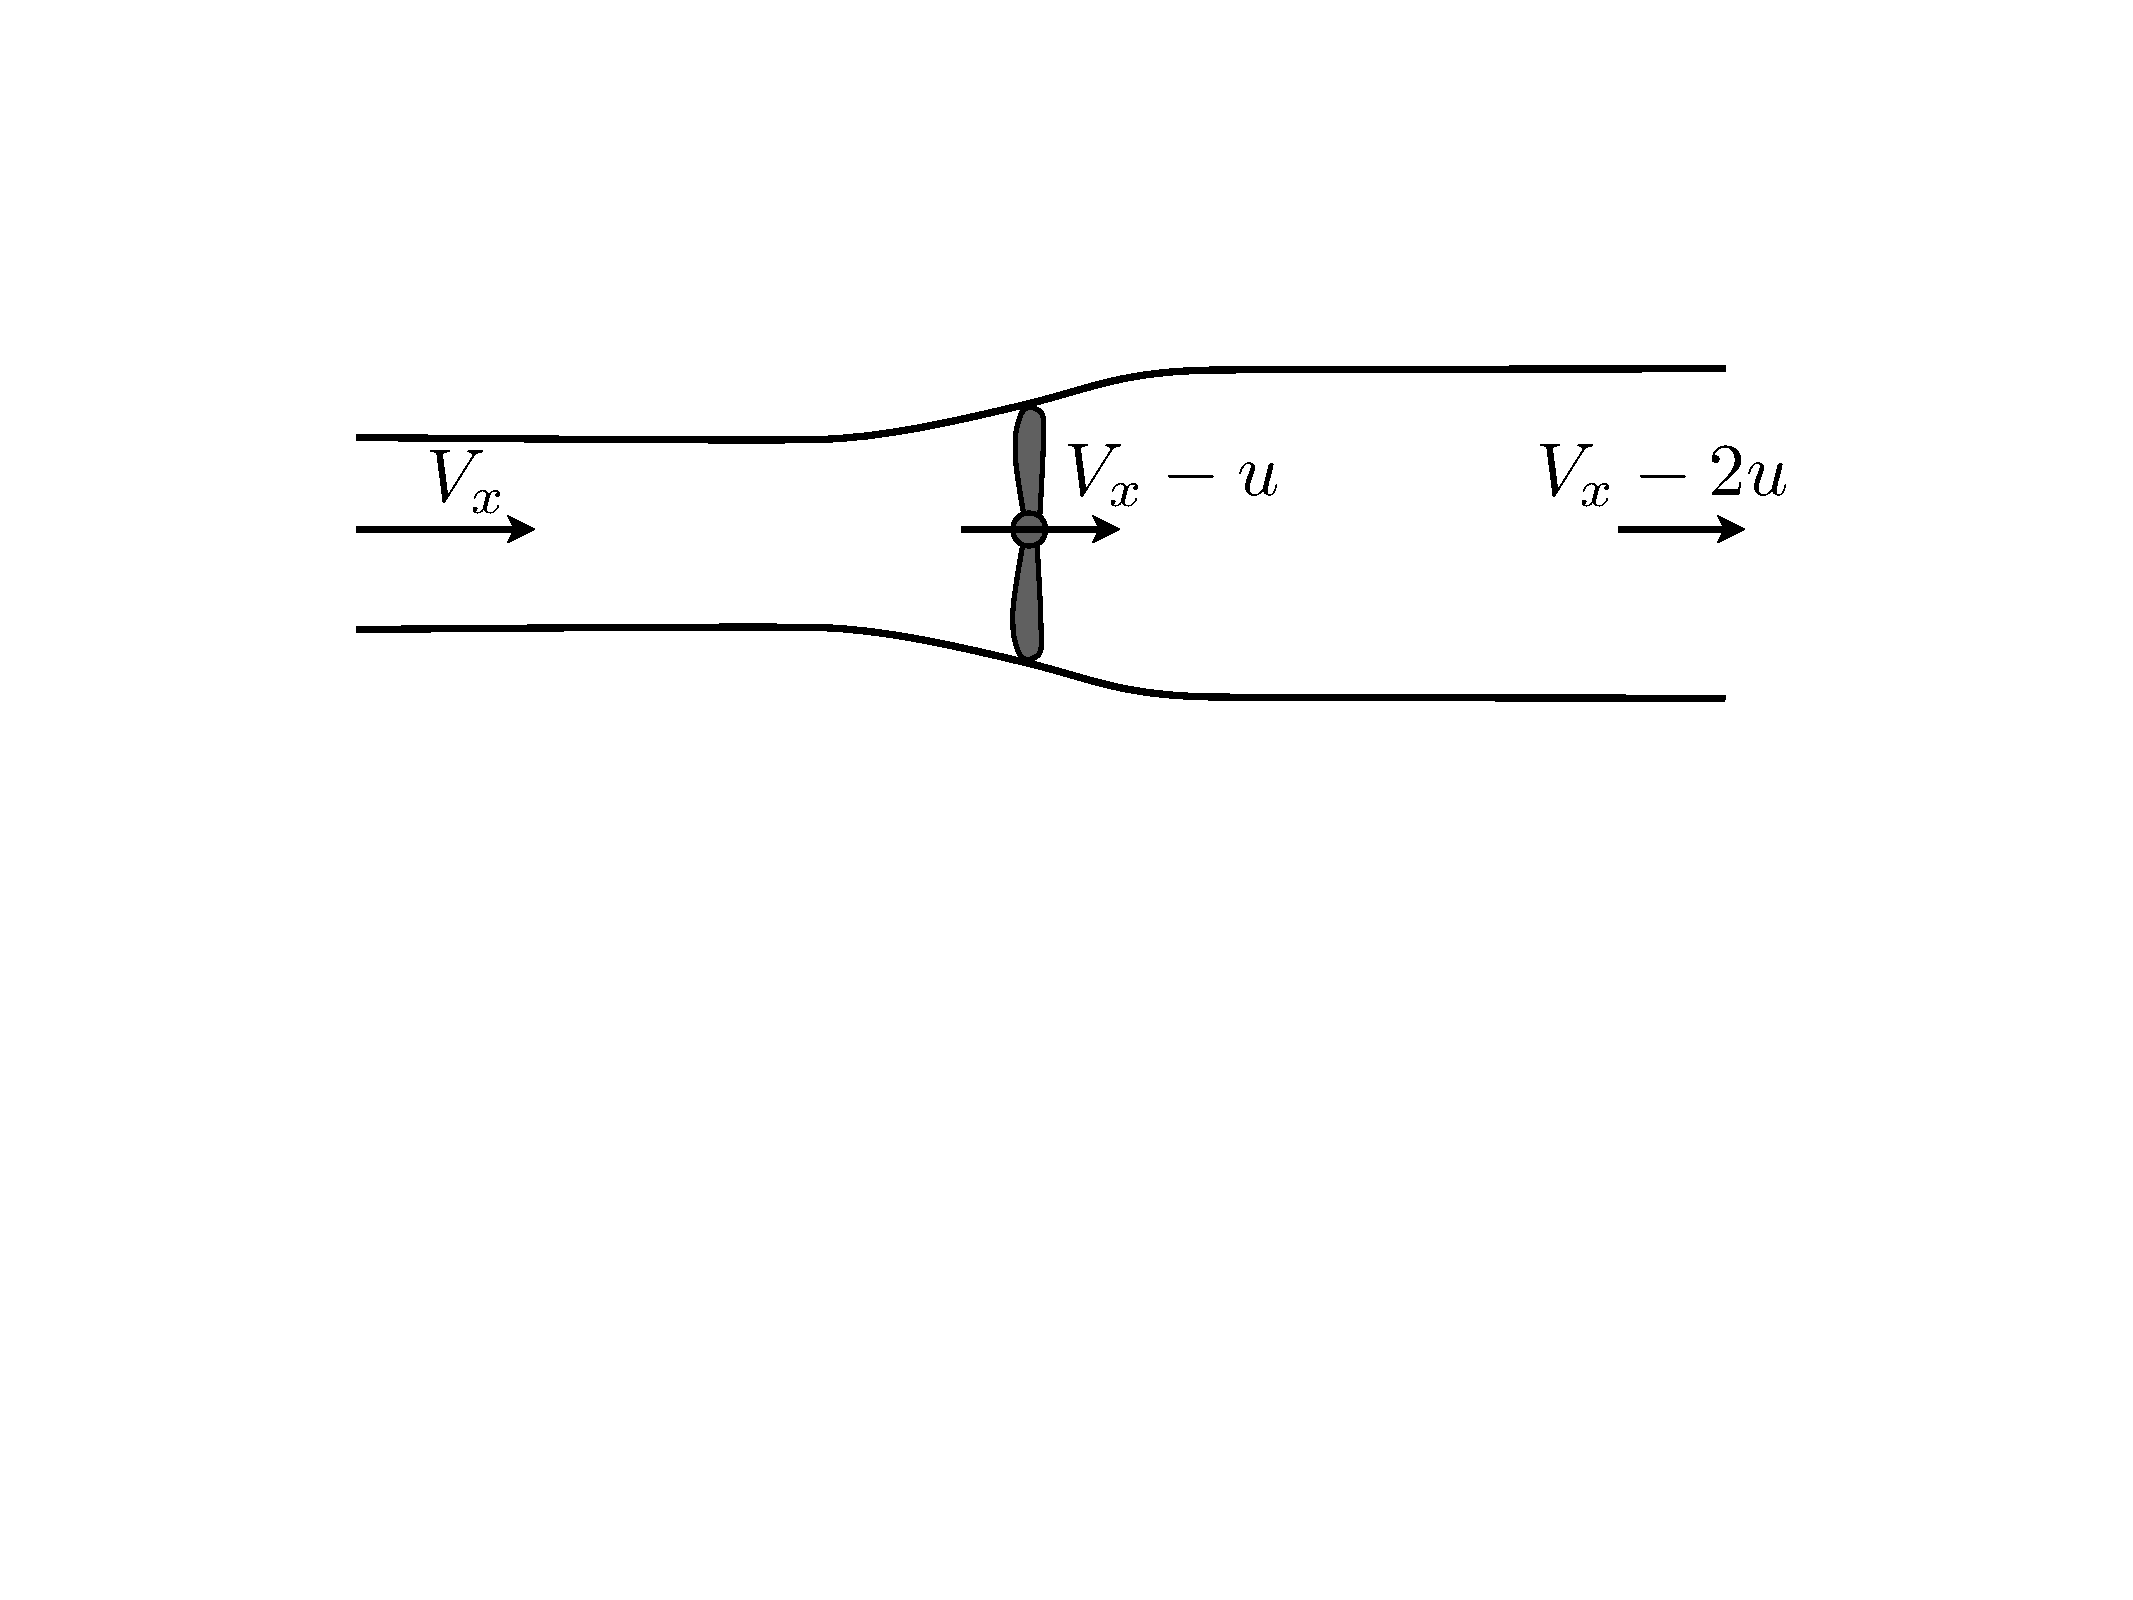
\includegraphics[width=3.5in]{figures/velocity-deficit1}
\caption{}
\label{fig:velocity-deficit}
\end{figure}
By convention we nondimensionalize $u$ as follows
% (where we call $V_1$ the freestream velocity $V_\infty$ by convention):
\begin{equation}
\begin{aligned}
V_2 &= V_x - u\\
&= V_x\left(1 - \frac{u}{V_x}\right)\\
&= V_x\left(1 - a\right)\\
\end{aligned}
\label{eq:V2}
\end{equation}
The quantity $a$ is called the axial induction factor.  Similarly, we can express the far-field velocity as:
\begin{equation}
    V_4 = V_x(1 - 2a)
    \label{eq:V4}
\end{equation}

The thrust can also be expressed in terms of the axial induction factor (using \cref{eq:thrust2,eq:momentum1,eq:V2,eq:V4}):
\begin{equation}
\begin{aligned}
    T &= \rho A_2 V_2 (V_x - V_w)\\
    T &= \rho A_2 V_x(1-a) (V_x - V_x(1-2a))\\
    T &= \rho A_2 V_x^2 2a (1-a) \\
\end{aligned}
\label{eq:momT}
\end{equation}
Finally, we nondimensionalize this expression to form the thrust coefficient.  We use $V_x$ as the reference velocity, and the local annulus area as the reference area.
\begin{equation}
\begin{aligned}
    C_T &= \frac{T}{\frac{1}{2}\rho V_x^2 A_2}\\
     &= 4 a (1 - a)
    \label{eq:CTmom}
\end{aligned}
\end{equation}

\subsection{Extensions and Modifications to the Basic Methodology}

Extensions and modifications applicable to momentum theory include: hub and tip losses, high induction factors, off-design wind directions, and propeller operation.  Each of these considerations is discussed below.

\subsubsection{Hub and Tip Losses}

The basic momentum theory ignores the hub and tip vortices that affect the induced velocity.  Various correct methods exist; we use the simple analytical expression developed by Prandtl\cite{Glauert1935-Airplane-Propellers}.
\begin{equation}
    \begin{aligned}
    f_{tip} &= \frac{B}{2} \left(\frac{R - r}{r|\sin\phi|} \right)\\
    F_{tip} &= \frac{2}{\pi} \arccos(\exp(-f_{tip}))\\
    f_{hub} &= \frac{B}{2} \left(\frac{r - R_{hub}}{R_{hub}|\sin\phi|} \right)\\
    F_{hub} &= \frac{2}{\pi} \arccos(\exp(-f_{hub}))\\
    F &= F_{tip}F_{hub}
    \end{aligned}
\end{equation}
The absolute value is necessary because our definition permits both positive and negative inflow angles.  This hub/tip-loss factor (which is always between 0 and 1) is applied directly to the thrust coefficient.
\begin{equation}
    C_T = 4 a (1 - a) F
    \label{eq:CTmom2}
\end{equation}

\subsubsection{High Induction Factors}

Empirical data suggests that this simple momentum model breaks down for large inductions.  The current expression for thrust coefficient (\cref{eq:CTmom2}) predicts a maximum at $a = 0.5$ as seen in \cref{fig:a}.  Additionally, this basic momentum derivation predicts a wake reversal in the far-field for axial induction factors larger than 0.5 (see \cref{eq:V4}).  This is non-physical, as the real flow entrains momentum in the wake through turbulence.  Empirical data suggests that the thrust coefficient continues to increase past induction factors of 0.5, all the way up to an axial induction factor of 1 (\cref{fig:a}).  Various simple extension methods exist, including the well-known quadratic fit from Glauert \cite{Glauert1926-General-Theory}.  However, the Glauert correction does not maintain C1 continuity when the tip/hub loss corrections are included.  Instead, we use a small modification of Glauert's method developed by Buhl \cite{Buhl2005-Empirical-Relationship}:
\begin{equation}
C_T = \left(\frac{50}{9} - 4F\right) a^2 - \left(\frac{40}{9} - 4F\right) a + \frac{8}{9} \qquad  0.4 \le a \le 1
\label{eq:CTBuhl}
\end{equation}

\begin{figure}[htbp]
\centering
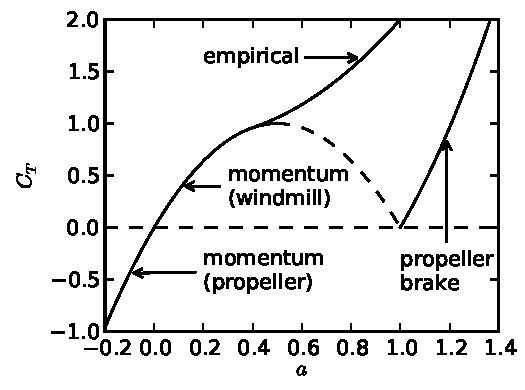
\includegraphics[width=3.5in]{figures/a}
\caption{Thrust coefficient as a function of axial induction factor.}
\label{fig:a}
\end{figure}

Additional considerations are needed for induction factors larger than 1, the so-called propeller brake region.  The current expression \cref{eq:CTmom2} predicts a negative thrust for induction factors larger than 1 (in other words, propeller operation).  However, repeating the momentum conservation, suggests that the thrust changes signs, in other words it still acts as a drag device.
\begin{equation}
    C_T = - 4 a (1 - a) F
    \label{eq:CTpb}
\end{equation}

% [TODO: show this]


\subsubsection{Other Wind Directions}

The above derivation is independent of the tangential, or in-plane velocities.  If the axial wind direction is reversed, nothing in the above derivation changes.  The positive thrust direction is still downwind, although because the ``downwind'' direction changes with a wind reversal, all of the thrust coefficients change sign if $V_x$ changes sign.  This is summarized in \cref{sec:momsum}.

\subsubsection{No Wind In One of the Directions}

Consider the case where $V_x = 0$.  As shown later, there is no tangential induction, but there is still an axially induced velocity.  However, we can no longer use the normalization $a = u/V_x$, because $V_x = 0$.  Instead, we must use the full induced velocity $u$.

Two scenarios are possible (\cref{fig:velocity-deficit2}).  No other scenario is possible, because the thrust and induction must be in opposite directions (see Kutta-Joukowski theorem and discussion in \cref{sec:be}).  These cases are analogous to a helicopter in hover.
\begin{figure}[htbp]
\centering
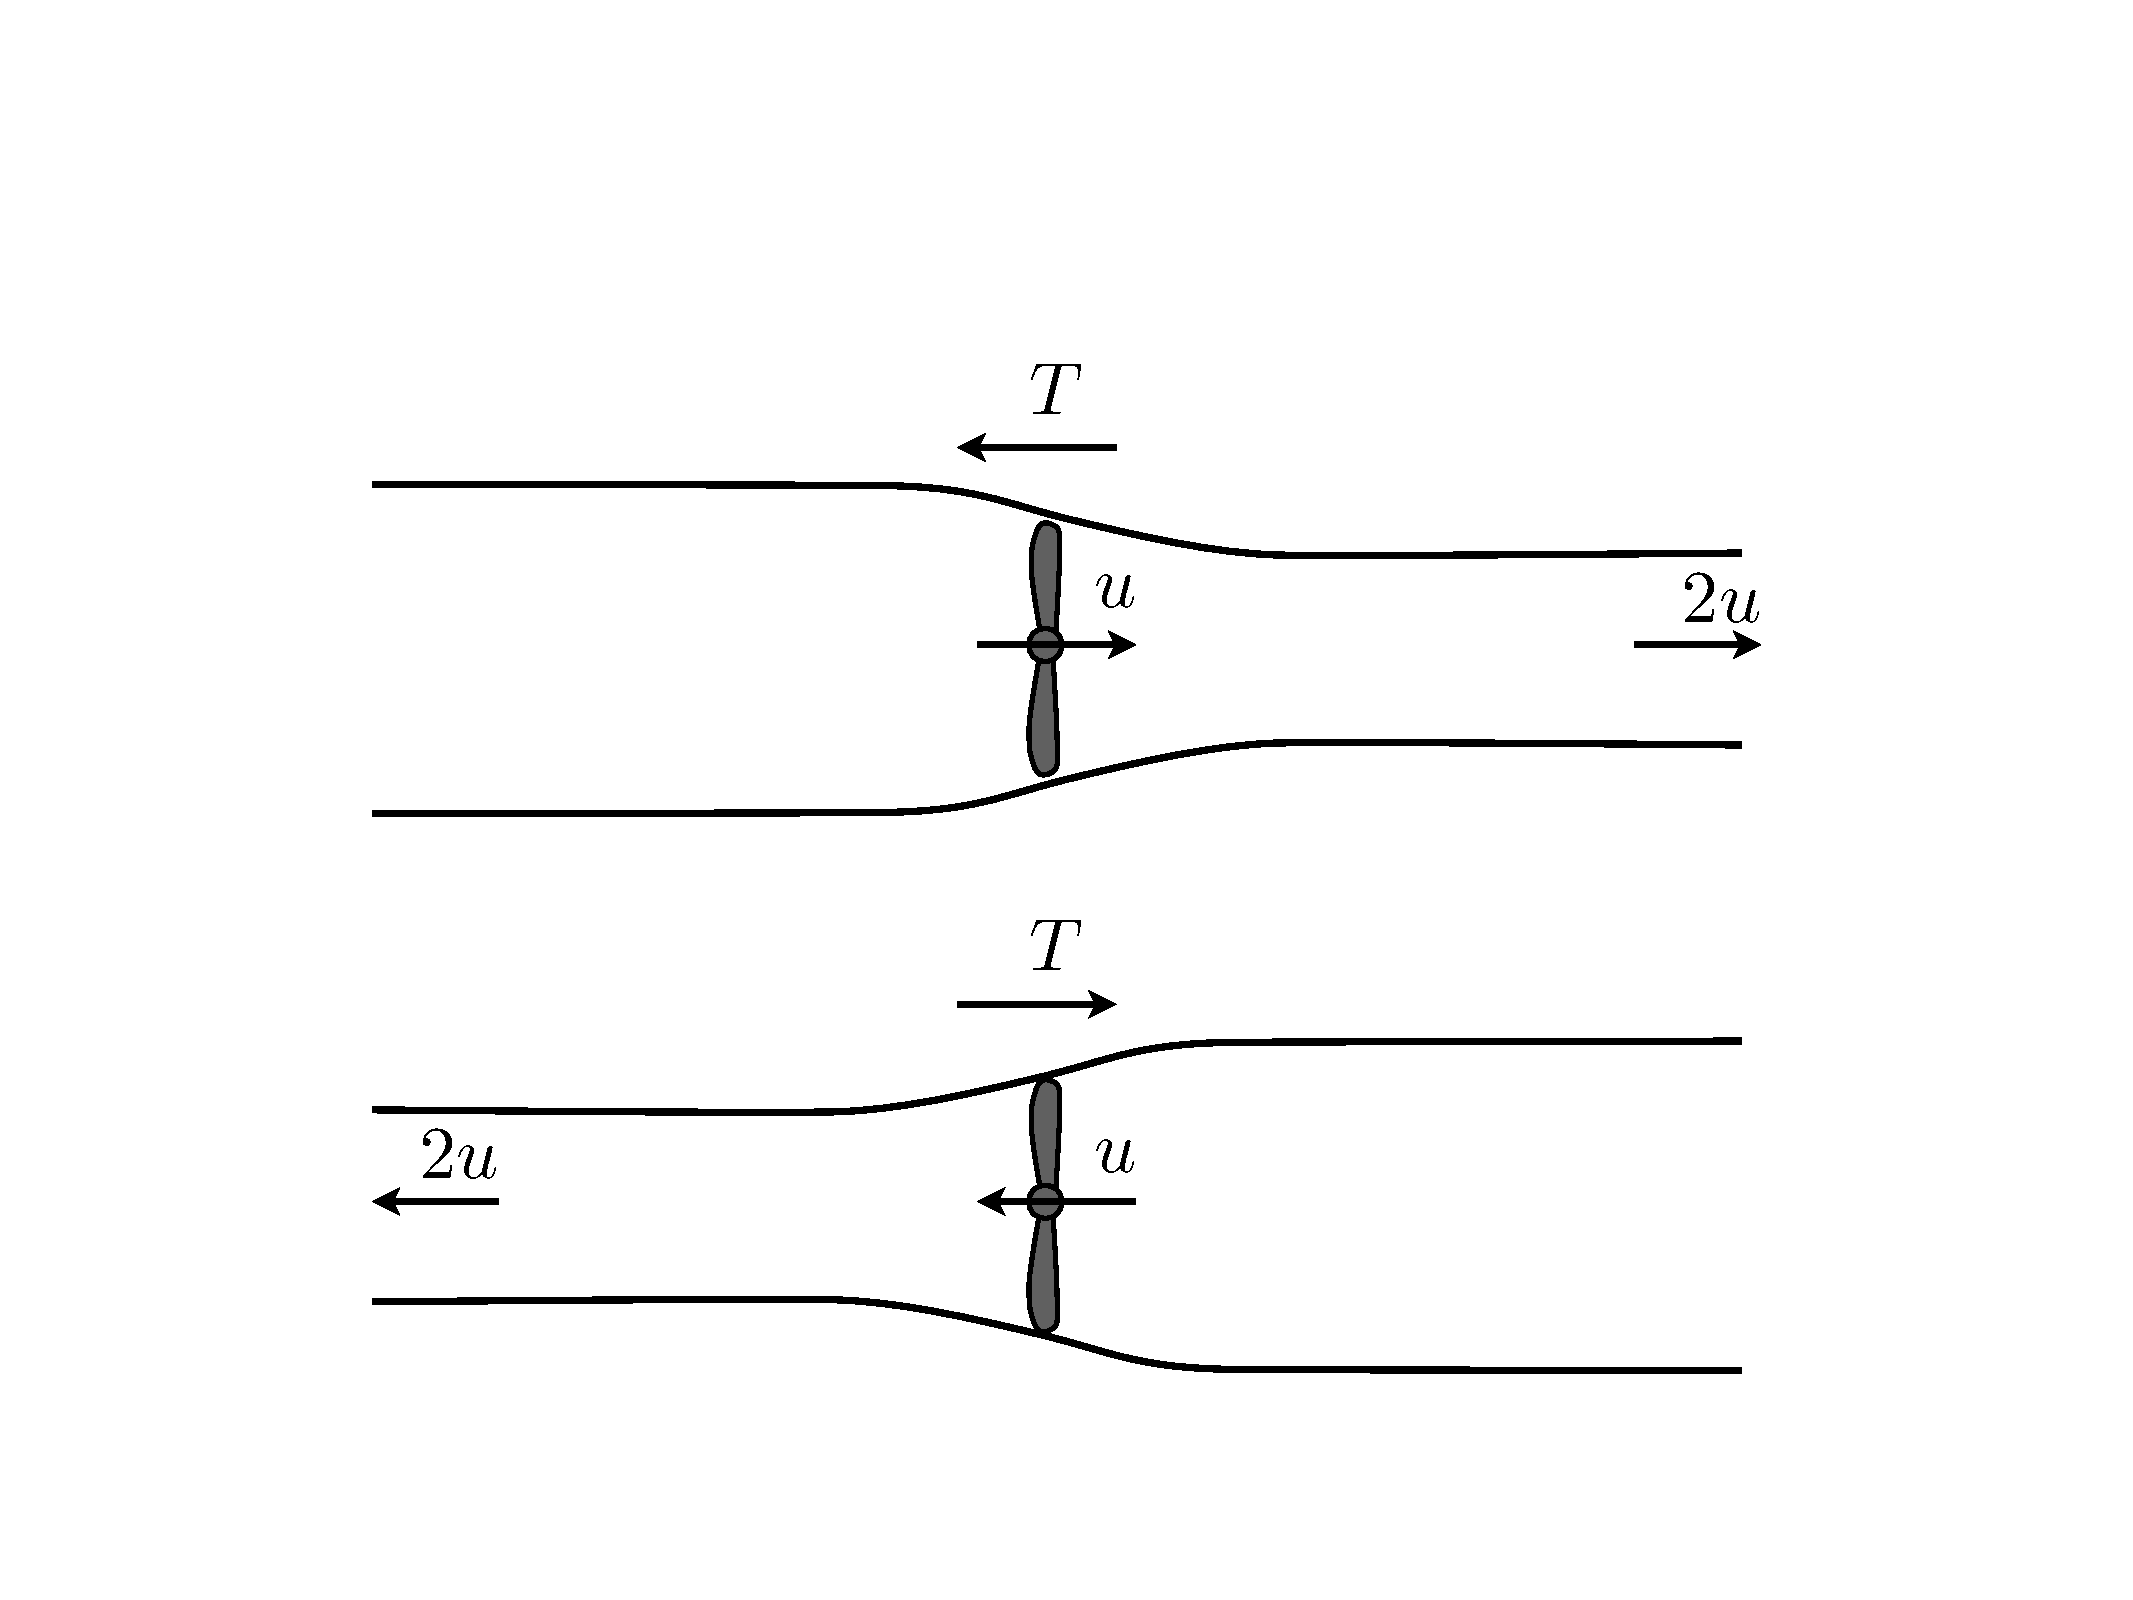
\includegraphics[width=3.5in]{figures/velocity-deficit2}
\caption{}
\label{fig:velocity-deficit2}
\end{figure}

Using \cref{eq:momT}, before the induction factor is introduced, we see that
\begin{equation}
    \begin{aligned}
        T &= -\rho A_2 V_2 V_w\\
        T &= -\rho A_2 (-u) (-2u)\\
        T &= - 2 \rho A_2 u^2\\
    \end{aligned}
\end{equation}
Using the area of the annulus and the hub/tip loss factors results in
\begin{equation}
    T = - 4 \pi r \rho u^2 F dr\\
\end{equation}
We do not nondimensionalize this thrust, because $V_x = 0$, but do need to consider the sign.  We define the positive convention for $u$, as consistent with our positive convention for $a$.  In other words, a positive $u$ is in the $-x$ direction.  Thus, our equation for thrust becomes:
\begin{equation}
    T =
    \begin{cases}
    4 \pi r \rho u^2 F dr & u > 0\\
    -4 \pi r \rho u^2 F dr & u < 0\\
    \end{cases}
\end{equation}

If $V_y = 0$, then there is no axially induced velocity ($a = 0$), and $V_x$ passes through unchanged. Momentum theory predicts no thrust.  There is actually thrust, from the drag on the blades, but this arises from blade element theory and is treated later.




\subsubsection{Propellers}

Nothing in the above derivation needs to be changed to handle propeller analysis.  The only physical change is that the propeller imparts energy to the fluid and so the induced velocity adds to the freestream velocity, rather than subtracts from it.

In a conventional propeller derivation we would change the sign of the induced velocities, and change the conventional positive direction for thrust, and thus write the thrust coefficient as:
\begin{equation}
    C_T = 4 a (1 + a) F
\end{equation}
However, if we keep the conventions consistent we can use the exact same equations we have already derived.  If $a$ is negative that means the sign of the induced velocity has changed and is thus operating as a propeller.  Our existing expression for thrust coefficient \cref{eq:CTmom2} gives then the correct result for a negative $a$:
\begin{equation}
    C_T = - 4 a (1 + a) F
\end{equation}
Because we are keeping our positive convention as a positive thrust downwind, this correctly predicts the thrust as occurring upwind while in propeller operation.  In summary, we can use \cref{eq:CTmom2} for either turbines or propellers.

\subsection{Summary}
\label{sec:momsum}

\begin{equation}
\begin{aligned}
    V_x > 0:&\quad
    C_T =
    \begin{cases}
        4 a (1 - a) F &  a \le 0.4 \\
        \left(\frac{50}{9} - 4F\right) a^2 - \left(\frac{40}{9} - 4F\right) a + \frac{8}{9} &  0.4 < a < 1 \\
        -4 a (1 - a) F &  a \ge 1 \\
    \end{cases}\\
    V_x < 0:&\quad C_T \text{ has the opposite sign of above}\\
    V_x = 0:&\quad  T =
        \begin{cases}
        4 \pi r \rho u^2 F dr & u > 0\\
        -4 \pi r \rho u^2 F dr & u < 0\\
        \end{cases}\\
    V_y = 0:&\quad T = 0\\
\end{aligned}
\label{eq:CTmomsum}
\end{equation}

% Otherwise, if $V_x < 0$, then $C_T$ has the opposite sign.
%
% If $V_x = 0$ then
% \begin{equation}
%
% \end{equation}
% and if $V_y = 0$, no thrust is predicted from momentum theory.


% The positive direction of thrust for these derivations is the local downwind direction, in other words it is in the direction of the local axial component of velocity.


\section{Angular Momentum Balance}

Similar to the linear momentum case where an induced velocity is produced in opposition to the force on the rotor, the rotation of the blades is accompanied by a rotation of the fluid in the opposite direction to that of the rotor.  Unlike, the linear momentum case where the induced velocity change occurs across a large control volume, the rotational velocity change occurs only across the rotor disk. We define the tangential induction as $a^\prime = v/V_y$, where $v$ is the induced velocity in the $+y$ direction.  Conservation of momentum yields the same result as the linear case, where the induced at the disk is halfway between its upstream and downstream values.  Except in this case, upstream and downstream is just upstream and downstream of the rotor disk, instead of in the farfield.  The induced rotational velocity is 0 upwind of the rotor, $V_y a$ in the plane of the rotor, and $V_y 2 a^\prime$ downstream of the rotor (oppositing the direction of rotation).

An angular momentum balance across a given control volume can be expressed as:
\begin{equation}
    \int_S \left(\vec{r} \times \vec{V}\right) \dot{m} = \sum \vec{Q}
\end{equation}
We use a disk-shaped control volume that surrounds the rotor disk, and assume no axial component of velocity exists on the sides of the control volume.  We are then interested in only the inflow and outflow velocity vectors into the control volume. \Cref{fig:wtvt} uses an ground-centered inertial control volume, rather than a blade-centric control volume to show the velocity triangles.  This is a somewhat unconventional frame of reference and orientation for a wind turbine, but is commonly used in turbomachinery analysis, and is convenient for this particular analysis.  In this figure, $v_w$ is the y-component of wind (or apparent wind resulting from blade-motion), and $V_y = \Omega r + v_w$.
\begin{figure}[htbp]
\centering
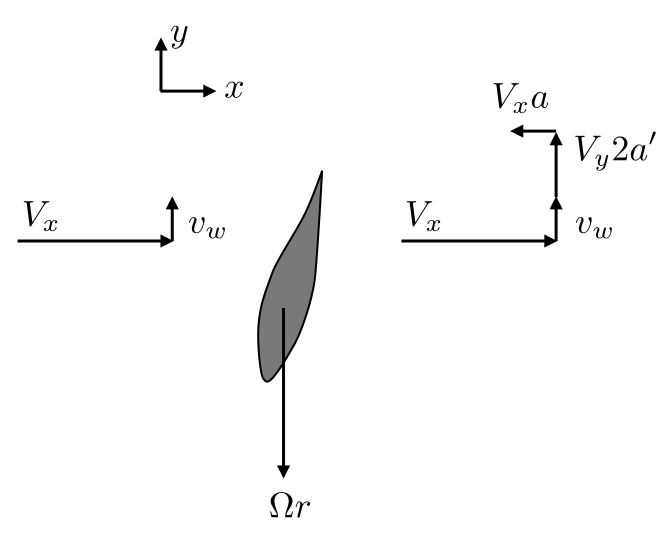
\includegraphics[width=3.0in]{figures/wtvt}
\caption{}
\label{fig:wtvt}
\end{figure}

% [TODO: discuss where $a^\prime$ comes from and the factor of 2]

Applying conservation of angular momentum yields (where we define positive torque on the rotor as positive in the $+x$ direction):
\begin{equation}
    \begin{aligned}
        r v_w \dot{m} - r (v_w + V_y 2 a^\prime) \dot{m} = -Q\\
         r V_y 2 a^\prime \dot{m} = Q\\
    \end{aligned}
    \label{eq:momQ}
\end{equation}

Using the results from the previous section:
\begin{equation}
    \dot{m} = \rho V_2 A_d = \rho V_x(1-a) A_d
    \label{eq:mdot}
\end{equation}
Thus:
\begin{equation}
    Q = 2 r V_y a^\prime \rho V_x(1-a) A_d
\end{equation}

% (TODO: note that the results for linear momentum stay the same even when assuming a swirl)

As we did for thrust, we normalize to form the torque coefficient using $V_x$ as the reference velocity, and the annulus area as the reference area.
\begin{align}
    C_Q &= \frac{Q}{\frac{1}{2}\rho V_x^2 A_d r}\\
     &= 4 a^\prime (1-a) \frac{V_y}{V_x}
\end{align}
% \begin{align*}
%     C_Q &= \frac{Q}{\frac{1}{2}\rho V_\infty^2 A_d r}\\
%      &= 4 a^\prime (1-a) \frac{V_x V_y}{V_\infty^2}
% \end{align*}

\subsection{Extensions and Modifications to the Basic Methodology}

The same set of extensions and modifications are considered for torque, as they were for thrust.

\subsubsection{Hub/Tip Losses}

The torque correction is the same approach as is used for thrust, where the hub/tip loss factor $F$ is multiplied against the torque.

\subsubsection{Other Wind Directions}

If the direction of $V_x$ reverses, then nothing in the above derivation changes.  We note that only component of velocity that matters is the induced velocity: $V_y 2 a^\prime$.  If $V_x$ reverses, then the induced velocity $V_y 2 a^\prime$ switches to the other side of the airfoil, but still points upward.  Because the direction of the velocity is the same, the $\vec{r} \times \vec{V}$ retains the same sign, and the mass flow is still on the ``out'' side of the control volume and also retains the same side.  However, because $V_x$ appears in our formula, and has switched signs itself, we need to add a negative sign so that the overall sign for $C_Q$ remains unchanged.

% The positive direction for torque also changes, but that changes signs for both sides of the equation and in the end nothing is changed.

If $V_y$ changes sign, either because the blades rotate backwards, or because the local wind $v$ becomes large in magnitude and negative, then the direction for the induced velocity $V_y 2 a^\prime$ changes direction as well.  In that case, there is a change in sign for the $\vec{r} \times \vec{V}$ term.  The torque coefficient changes signs, but is otherwise unaffected.  Because $V_y$ appears in the above equation, that sign change is taken care of automatically.

\subsubsection{No Wind In One of the Directions}

If $V_x = 0$, then there is no induced velocity in the tangential direction ($a^\prime = 0$).  In that case, no torque is predicted from momentum theory, but some torque may be generated from blade element theory as will be treated later.

If $V_y = 0$, then there is no induced velocity in the axial direction ($a = 0$).  There is induced velocity in the tangential direction, but we can not use the normalization for $a^\prime = v/V_y$ because $V_y = 0$.  Instead, we refer to the total induced velocity in the plane of the rotor as $v$.  The resulting torque from \cref{eq:momQ} and \cref{eq:mdot} is:
\begin{equation}
    \begin{aligned}
        r v_w \dot{m} - r (v_w + 2 v) \dot{m} &= -Q\\
        2 r v \dot{m} &= Q\\
        Q &= 2 r v \rho V_x A_d\\
    \end{aligned}
\end{equation}
We can normalize, because $V_x \ne 0$, but it will be convenient to keep this expression in the nonnormalized form.  We do, however, need to add the hub/tip loss factor
% Then, the torque coefficient is (we can still normalize because $V_x \neq 0$), and adding in the hub/tip loss factor:
% \begin{equation}
% \begin{aligned}
%     C_Q &=  \frac{2 r v \rho V_x A_d R}{\frac{1}{2}\rho V_x^2 A_d r} = 4F \frac{v}{V_x}
% \end{aligned}
% \end{equation}
Note that this is the same expression, if we were to use the existing formula for $Q$ but use $a = 0$, and replace $V_y a^\prime$ with $v$.

The sign of $v$ is consistent with the sign of $Q$ automatically.  A positive $v$ is in the y-direction, as is consistent with the normal case where $v = V_y a^\prime$.  However, as discussed in the previous section, reversing the sign of $V_x$ must be accounted for (total sign of $Q$ stays the same, so we must multiply by $-1$ to cancel sign change for $V_x$).
\begin{equation}
    Q = \pm 4 \pi F r^2 v \rho V_x dr
\end{equation}



\subsubsection{Propellers}

As discussed previously, when $a$ becomes negative the rotor acts as a propeller, and that is accounted for automatically in the above analysis.  Similarly, for a propeller, the sign of $a^\prime$ reverses.  This reverses the direction of the torque (power must be input, rather than extracted), but this also is taken care of automatically in the above derivation.  In short, no changes are needed.

\subsection{Summary}

% \begin{equation}
%     C_Q =
%     \begin{cases}
%         4 F a^\prime (1-a) \frac{V_y}{V_x} &  V_x > 0 \\
%         - 4 F a^\prime (1-a) \frac{V_y}{V_x} &  V_x < 0 \\
%         4F \frac{v}{V_x} &  V_y = 0, V_x > 0 \\
%         -4F \frac{v}{V_x} &  V_y = 0, V_x < 0 \\
%         0 &  V_x = 0 \\
%     \end{cases}
%     \label{eq:CQmom}
% \end{equation}


\begin{equation}
\begin{aligned}
    V_y \ne 0:&\quad
    C_Q = \begin{cases}
        4 F a^\prime (1-a) \frac{V_y}{V_x} &  V_x > 0 \\
        - 4 F a^\prime (1-a) \frac{V_y}{V_x} &  V_x < 0 \\
    \end{cases}\\
    V_y = 0:&\quad
    Q = \begin{cases}
        4 \pi F r^2 v \rho V_x dr &  V_x > 0 \\
        -4 \pi F r^2 v \rho V_x dr &  V_x < 0 \\
    \end{cases}\\
    V_x = 0:&\quad Q = 0\\
\end{aligned}
\label{eq:CQmom}
\end{equation}

The positive direction of torque for this derivations is in the $+x$ direction.

\section{Blade Element Theory}
\label{sec:be}

Consider the airfoil section shown in \cref{fig:inflow1} with the positive directions for twist ($\theta$) defined as is conventional for a wind turbine.  The x and y axis are defined so that the z-axis is out of the page towards the direction of the blade tip.  We consider a general inflow of $V_x$ and $V_y$.  For an ideal condition $V_x = V_\infty$, and $V_y = \Omega r$, but because of wind and blade motion, we allow for any general velocity vectors.

\begin{figure}[htbp]
\centering
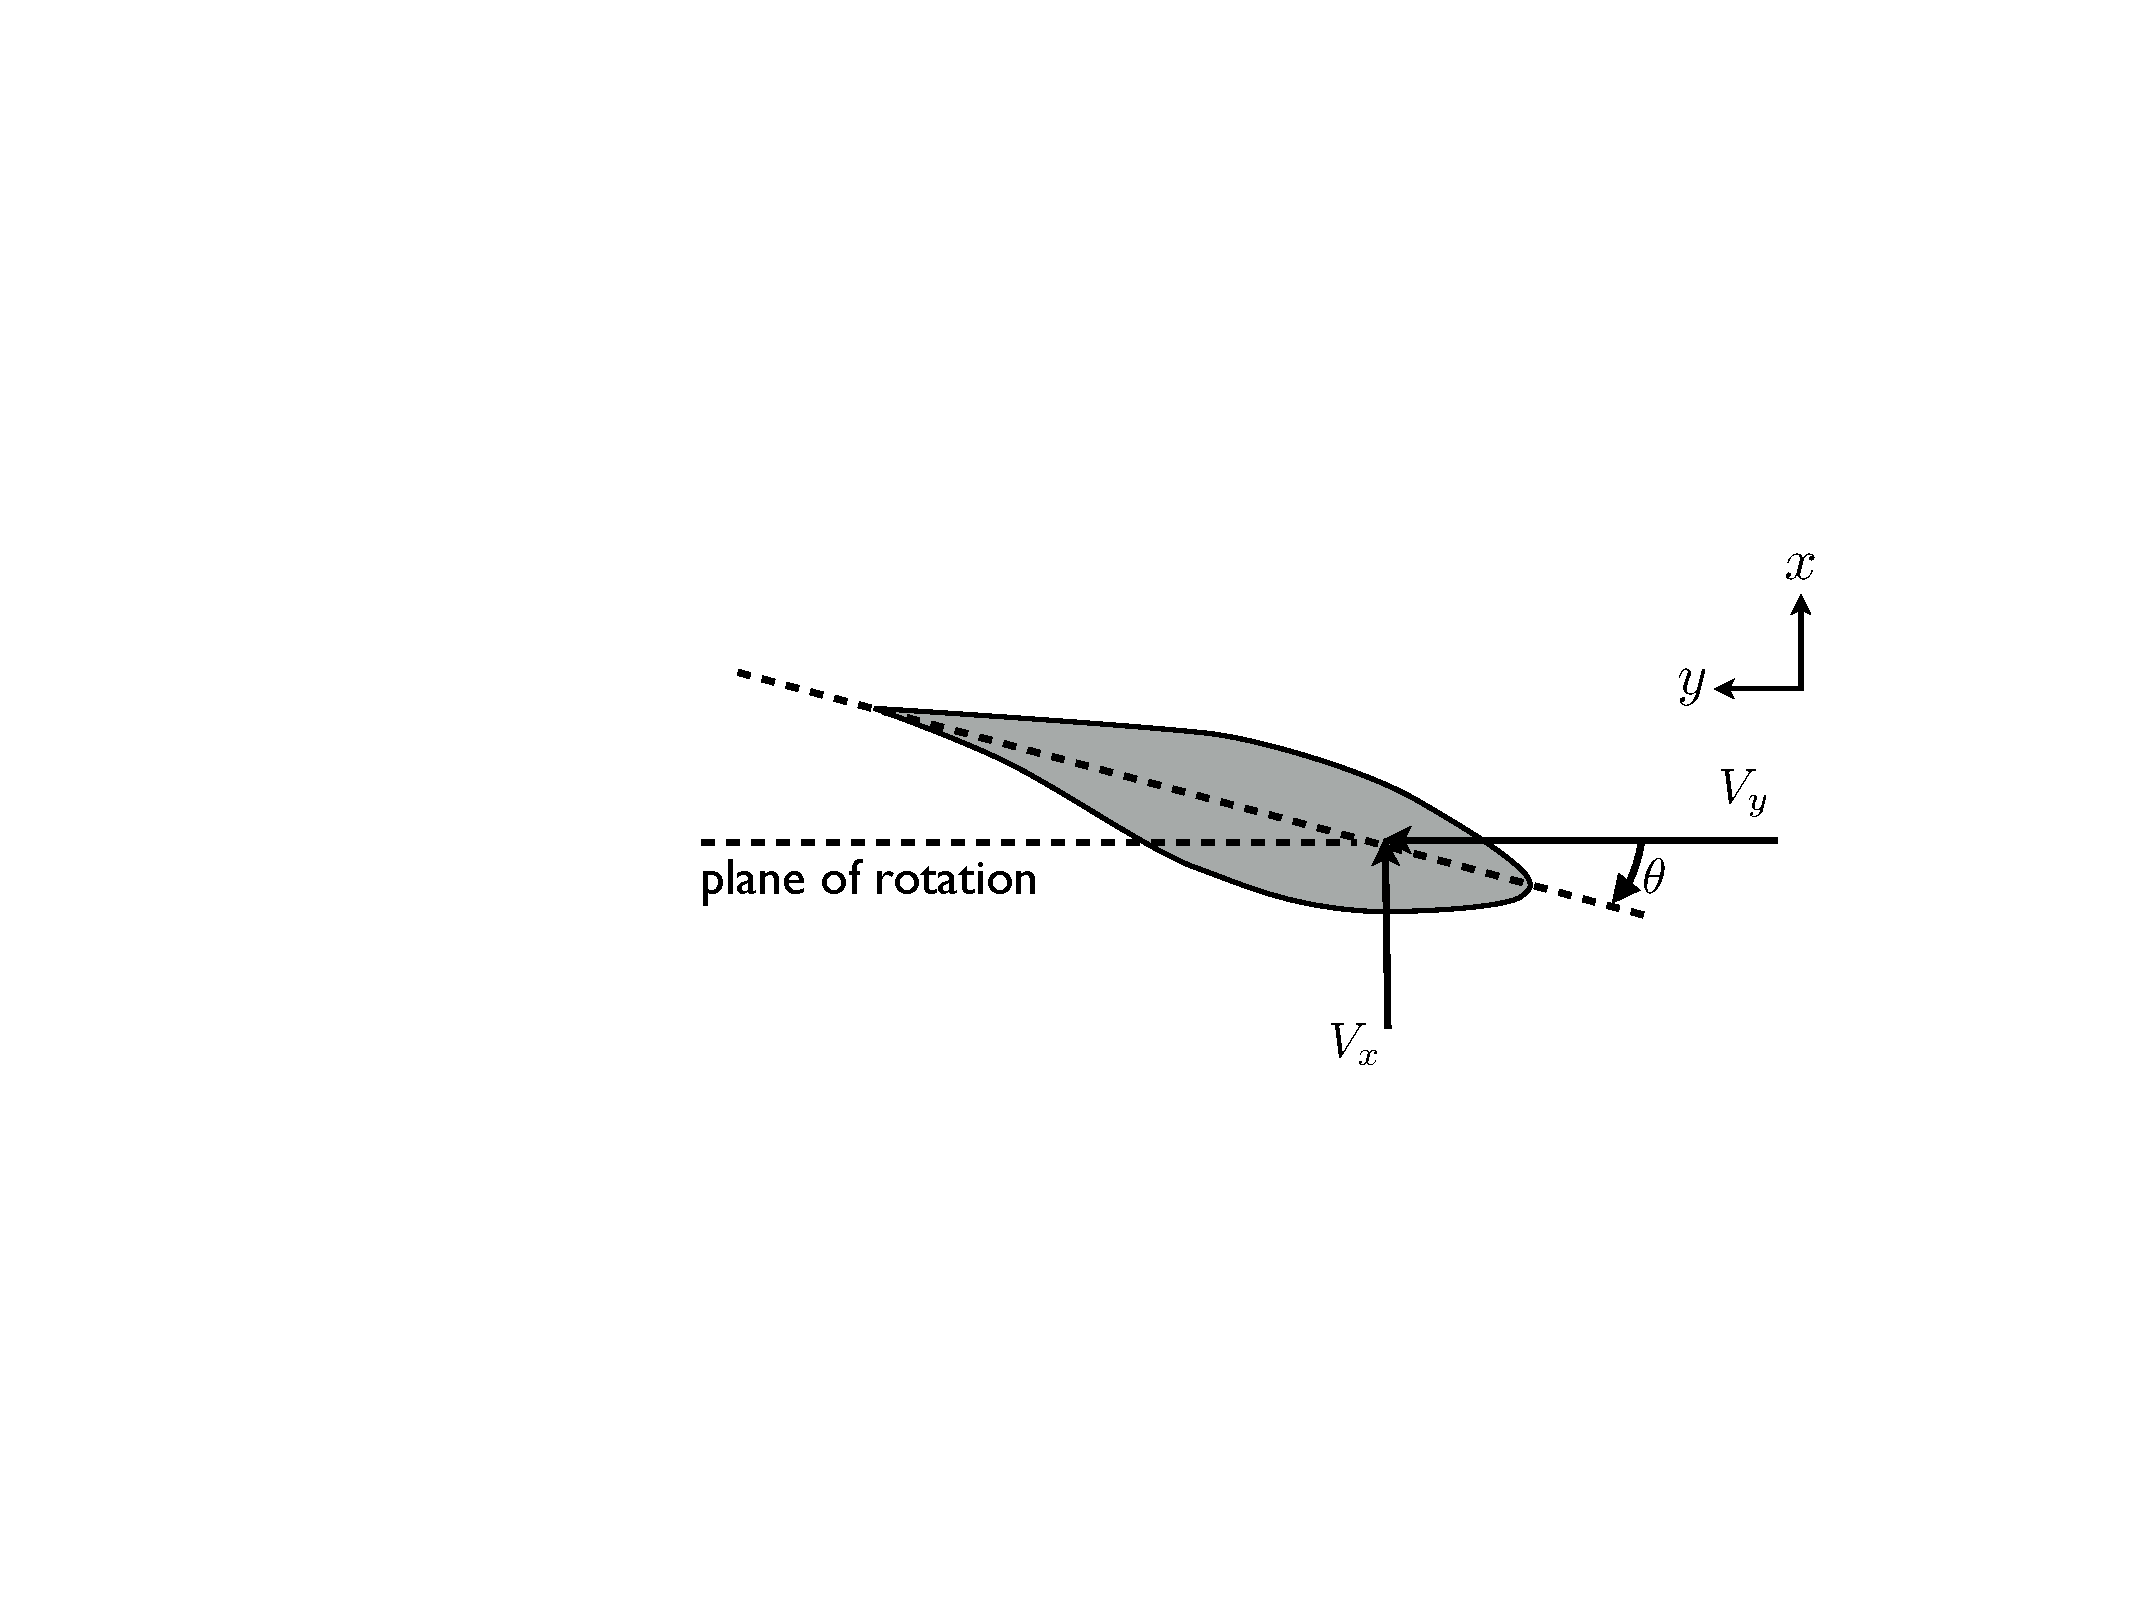
\includegraphics[width=3.5in]{figures/inflow1}
\caption{caption}
\label{fig:inflow1}
\end{figure}

For now, we assume that the airfoil is generating positive lift, as it would under normal operation (the solution will dictate the correct signs).  In that case, the direction of circulation $\Gamma$ is out of the page, and from the Kutta-Joukowski theorem:
\begin{equation}
    \vec{F}^\prime = \rho \vec{V} \times \vec{\Gamma}
\end{equation}
we can computed the resulting forces from the $V_x$ and $V_y$ components of velocity.  The resulting induced velocities oppose these forces.  For example, $V_x$ creates a force to the right, and thus an induced velocity to the left adding to that of $V_y$.  Conversely, $V_y$ creates a force upward, and thus an induced velocity downward opposing $V_x$.  As discussed previously, we normalize these induced velocities as follows: $a = u/V_x$ and $a^\prime = v/V_y$, where $u$ and $v$ are the x- and y-components of induced velocity respectively.  The resulting total inflow velocity vector $W$, positive direction for the inflow angle $\phi$, and angle of attack $\alpha$ are shown in \cref{fig:inflow2}.

\begin{figure}[htbp]
\centering
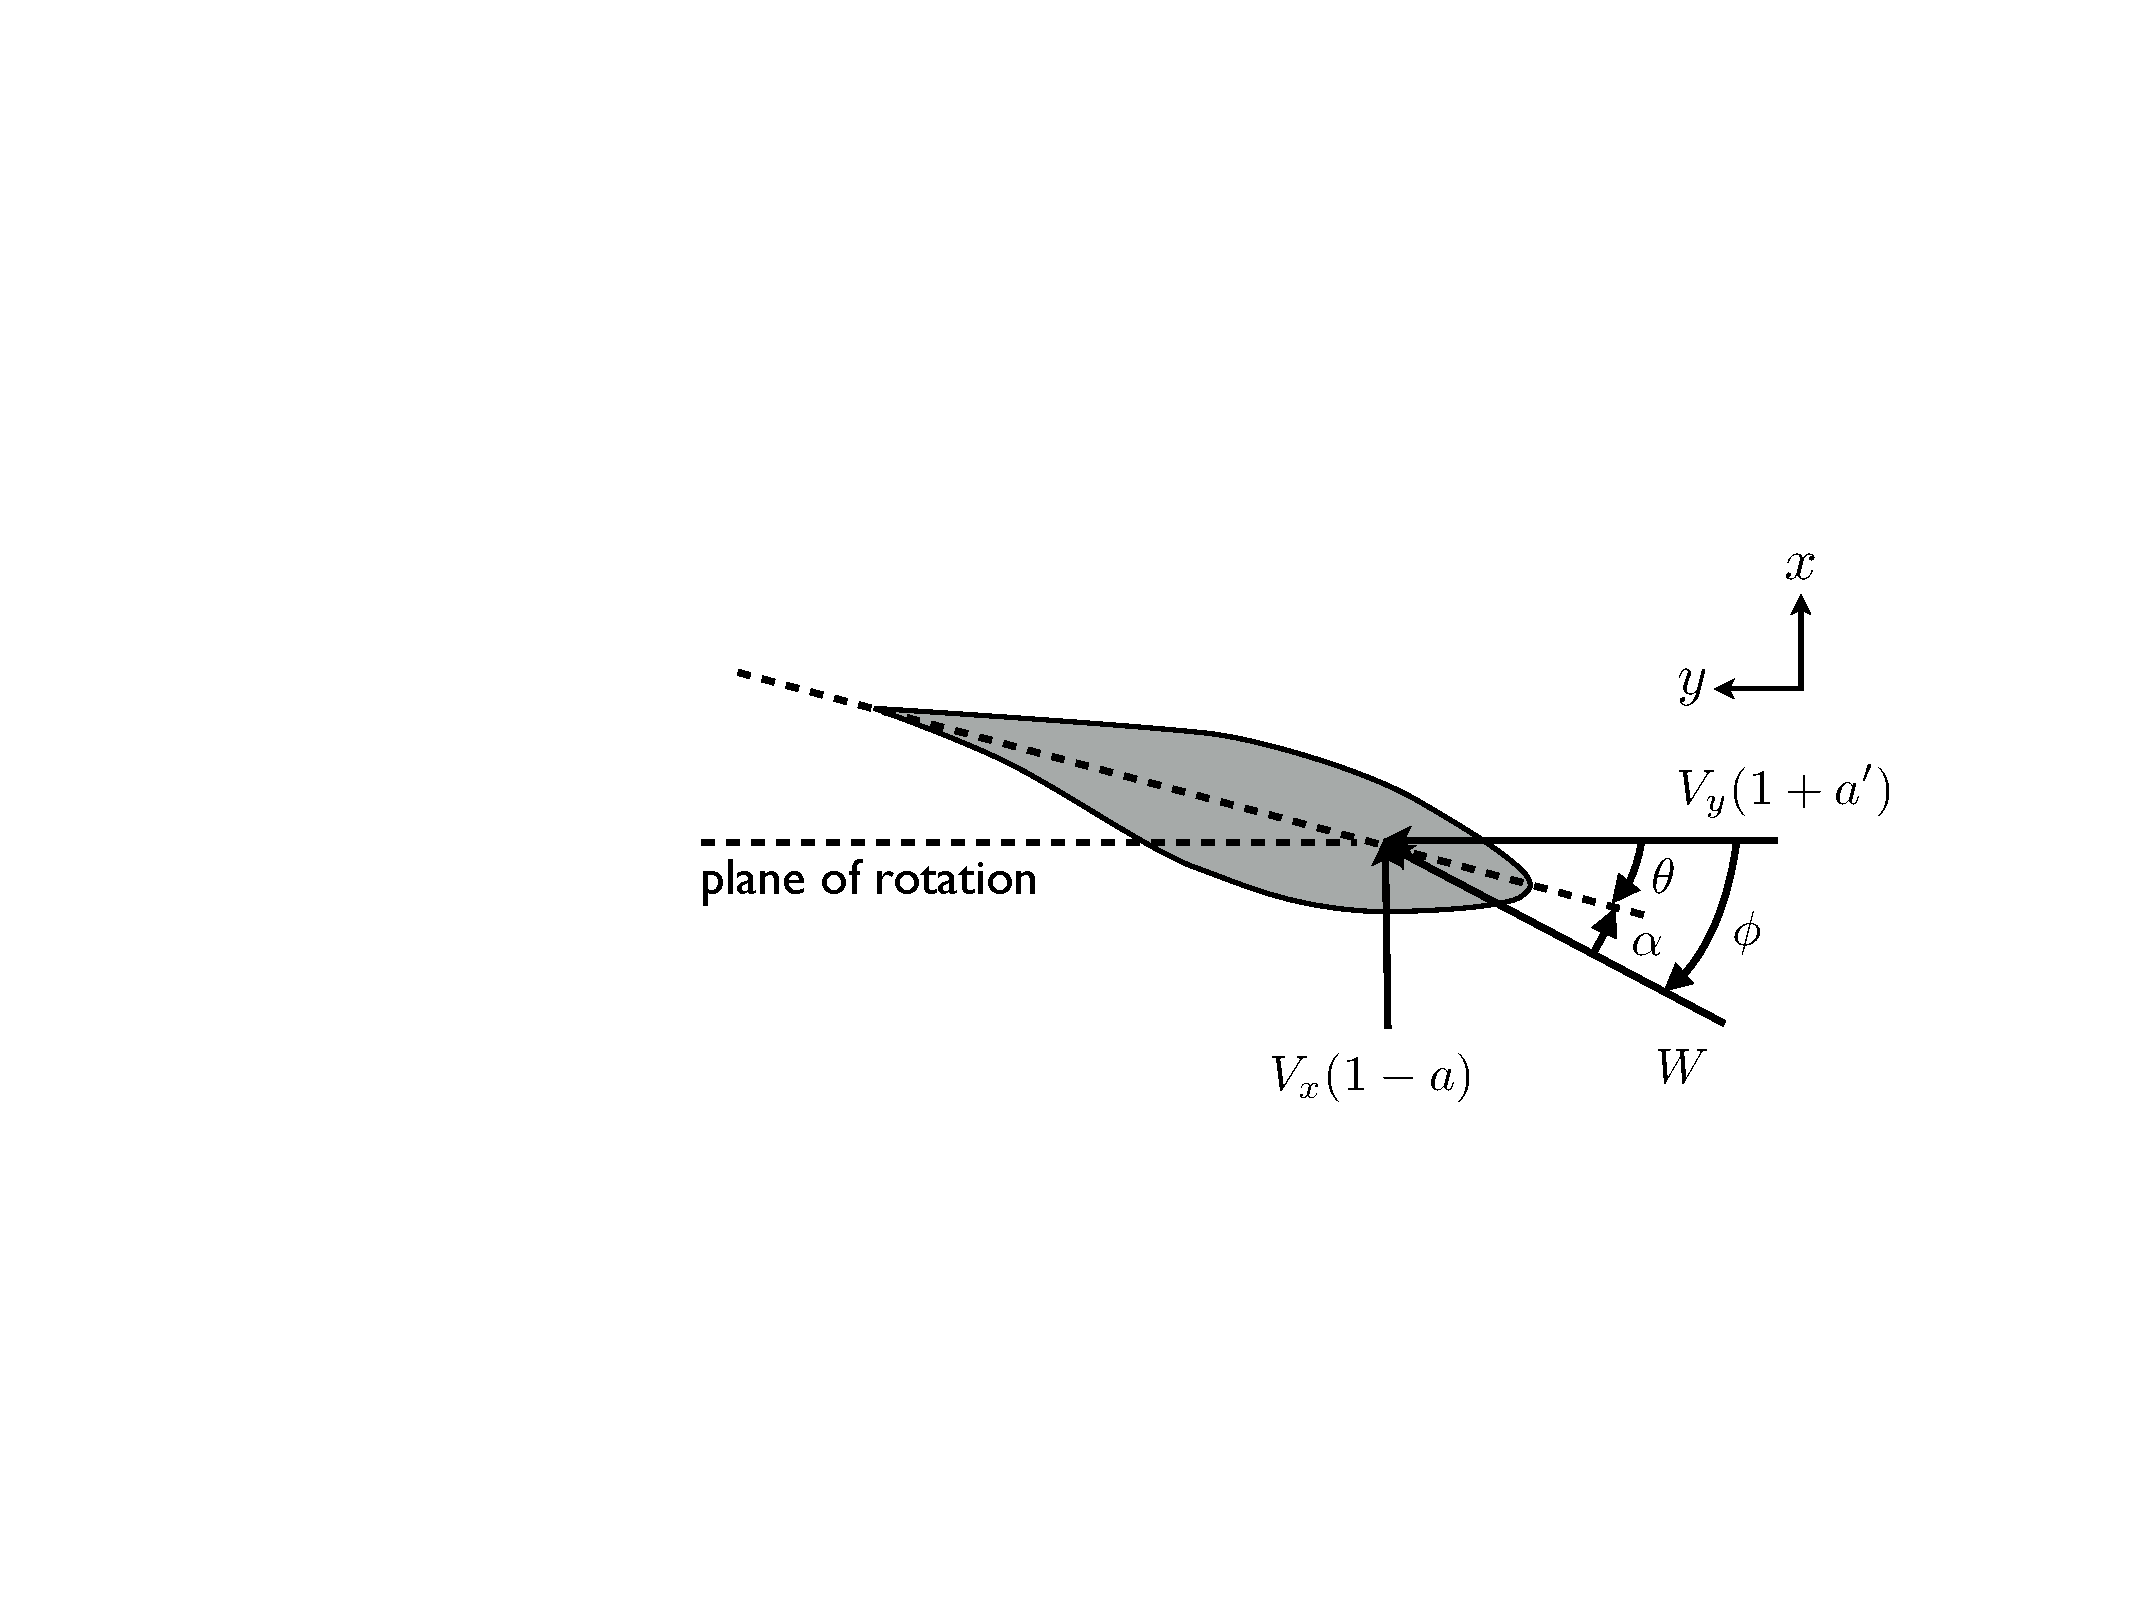
\includegraphics[width=3.5in]{figures/inflow2}
\caption{caption}
\label{fig:inflow2}
\end{figure}

From the definition of the angles we can relate the angle of attack, twist, and inflow angle:
\begin{equation}
    \alpha = \phi - \theta
    \label{eq:aoa}
\end{equation}
From the angle of attack we compute the sectional lift and drag coefficient.  To be core complete, the lift and drag coefficients are also functions of the Reynolds number.  Because we do not know $a$ and $a^\prime$ we usually approximate the Reynolds number using:
\begin{equation}
    \begin{aligned}
        W &= \sqrt{V_x^2 + V_y^2}\\
        Re &= \frac{\rho W c}{\mu}\\
    \end{aligned}
\end{equation}
The impact of this approximation is generally negligible.  First, inclusion of $a$ and $a^\prime$ generally only has a small effect on the Reynolds number.  Second, usually only order of magnitude changes in Reynolds number are important.  Third, airfoil data is usually not so precise that a minor change in Reynolds number is significant.  Still, if exactness in Reynolds number is needed, this can be achieved with one or two extra iterations \cite{Ning2014-Simple-Solution}.  We can now compute the lift and drag coefficients using any appropriate method (e.g., table look-up, a panel method, 2D RANS, etc.).  We denote these functions as $f_L$ and $f_D$.
\begin{equation}
    \begin{aligned}
        c_l &= f_L(\alpha, Re)\\
        c_d &= f_D(\alpha, Re)\\
    \end{aligned}
\end{equation}
Better implementations should account for unsteady aerodynamic airfoil behavior, and so the lift and drag coefficients are also functions of things like $\dot{\alpha}$, etc.

Using the Kutta-Joukowski theorem again, the directions for the lift and drag coefficients, $c_l$ and $c_d$ are as shown in \cref{fig:inflow3}.
\begin{figure}[htbp]
\centering
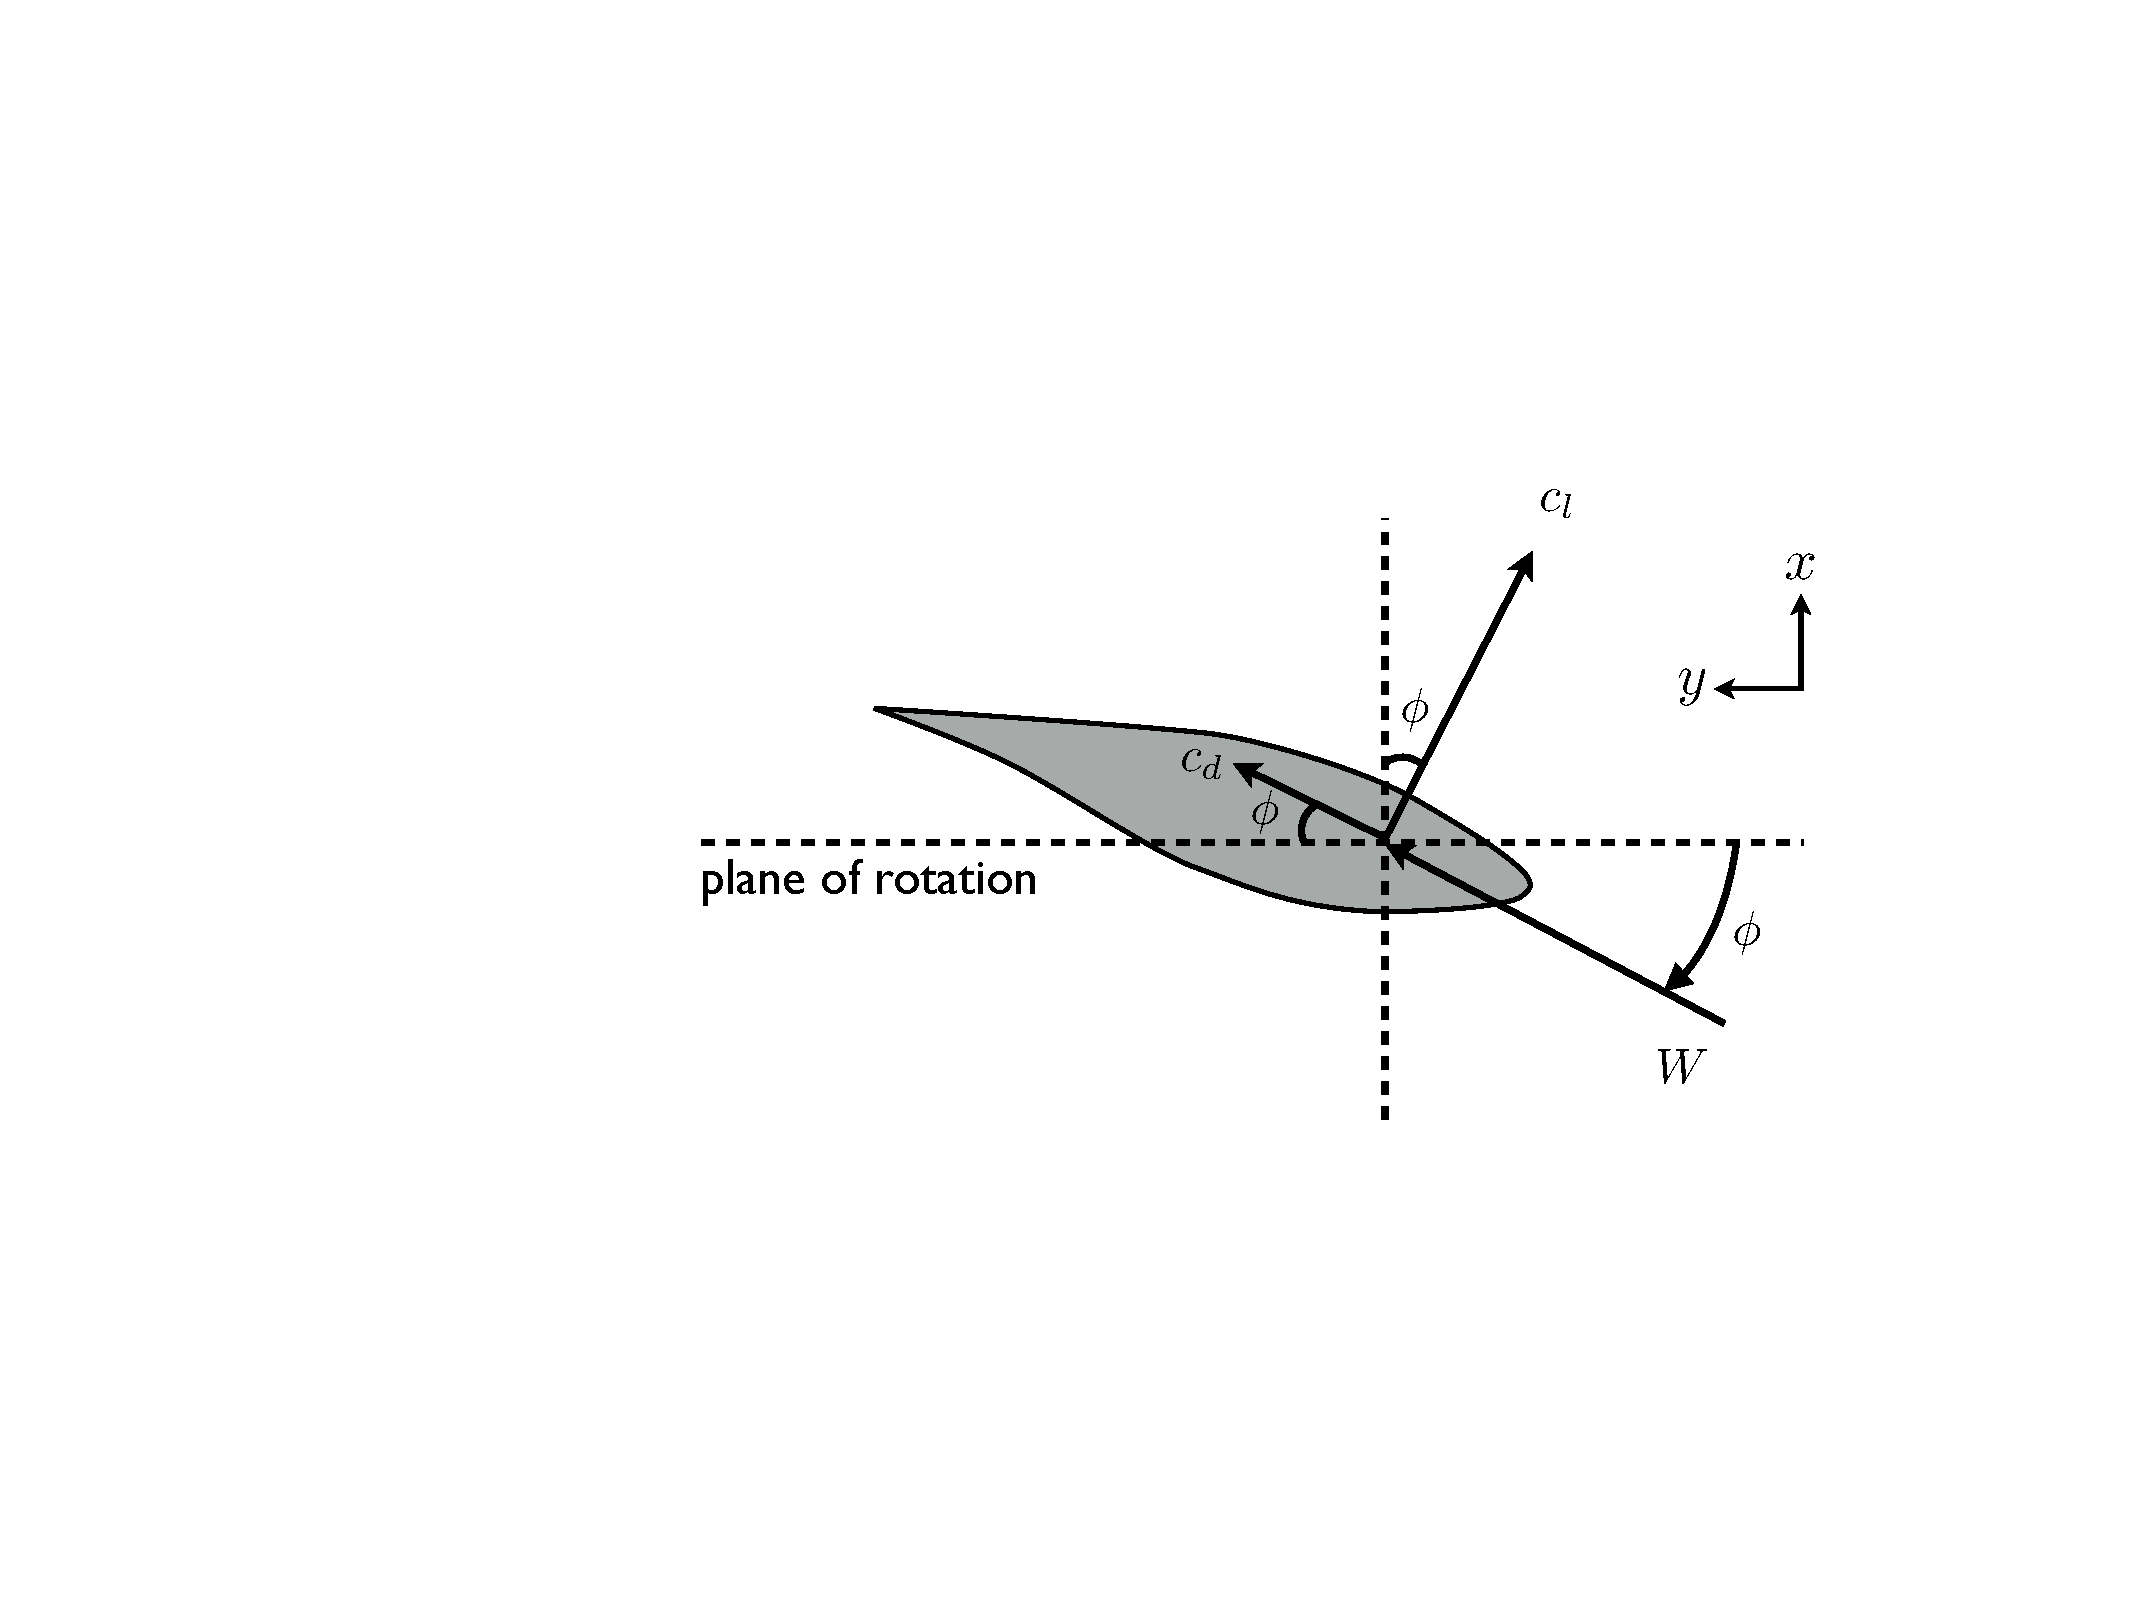
\includegraphics[width=3.5in]{figures/inflow3}
\caption{caption}
\label{fig:inflow3}
\end{figure}
We need to resolve these forces into the normal and tangential directions.  By convention, for wind turbines, we define the normal force coefficient $c_n$ in the direction of the +x-axis and the tangential force coefficient $c_t$ in the direction of the $-y$ axis (in the direction of blade rotation).
\begin{equation}
    \begin{aligned}
        c_n &= c_l \cos\phi + c_d \sin\phi\\
        c_t &= c_l \sin\phi - c_d \cos\phi\\
    \end{aligned}
\end{equation}

The total thrust and torque for this blade section, multiplied by the number of blades $B$ is:
\begin{equation}
    \begin{aligned}
        T = B N^\prime dr\\
        T = B c_n \frac{1}{2}\rho W^2 c dr\\
    \end{aligned}
    \label{eq:beT}
\end{equation}
\begin{equation}
    \begin{aligned}
        Q = B r T^\prime dr\\
        Q = B r c_t \frac{1}{2}\rho W^2 c dr\\
    \end{aligned}
    \label{eq:beQ}
\end{equation}
For normalization of thrust and torque coefficients we use the area of the affected annulus ($A = 2 \pi r dr$), and as the reference velocity in the dynamic pressure we will use the same one used in normalization in the momentum balances $q = 1/2 \rho V_x^2$.  Furthermore, we define the local solidity as:
\begin{equation}
    \sigma^\prime = \frac{B c}{2 \pi r}
\end{equation}
Performing the normalization results in:
\begin{equation}
    \begin{aligned}
        C_T &= \frac{T}{q_\infty A_d}\\
         &= c_n \sigma^\prime \left(\frac{W}{V_x}\right)^2\\
     \end{aligned}
 \end{equation}
 \begin{equation}
     \begin{aligned}
        C_Q &= \frac{Q}{q_\infty A_d r}\\
         &= c_t \sigma^\prime \left(\frac{W}{V_x}\right)^2\\
    \end{aligned}
\end{equation}

Ultimately, we want to relate this expression in terms of the induction factors.  Using \cref{fig:inflow2}, we see that
\begin{equation}
    W = \frac{V_x (1 - a)}{\sin \phi}
\end{equation}
or
\begin{equation}
    W = \frac{V_y (1 + a^\prime)}{\cos \phi}
\end{equation}

It will be convenient later to use the first substitution in the thrust coefficient, and one of each in the torque coefficient:
\begin{equation}
    C_T = c_n \sigma^\prime \left(\frac{1-a}{\sin\phi}\right)^2\\
    \label{eq:CTbe}
\end{equation}
\begin{equation}
    C_Q = c_t \sigma^\prime \left(\frac{1 + a^\prime}{\cos\phi}\right)\left(\frac{1 - a}{\sin\phi}\right)\left(\frac{V_y}{V_x}\right)
    \label{eq:CQbe}
\end{equation}
% \begin{equation}
%     C_T = c_n \sigma^\prime \left(\frac{1-a}{\sin\phi}\right)^2\left(\frac{V_x}{V_\infty}\right)^2\\
% \end{equation}
% \begin{equation}
%     C_Q = c_t \sigma^\prime \left(\frac{1 + a^\prime}{\cos\phi}\right)^2\left(\frac{V_y}{V_\infty}\right)^2\\
% \end{equation}

\subsection{Extensions and Modifications to the Basic Methodology}

Similar extensions and modifications must be made for blade element theory.

\subsubsection{Other Wind Directions}

It turns out that nothing in this derivation changes for other inflow directions, as long as we keep the definitions consistent (i.e., positive direction for $\phi$, $\alpha$, etc.).

% TODO: show this for some (or all) cases.

\subsubsection{No Wind In One of the Directions}
\label{sec:nowindtan}

If $V_x = 0$, then from the Kutta-Joukowski theorem, $a^\prime = 0$.  Also, $a$ is undefined, because of the normalization by $V_x$ and so we must refer to the total axial induced velocity $u$.  There are two possible directions for $u$ (\cref{fig:inflowu}).

\begin{figure}[htbp]
    \centering
    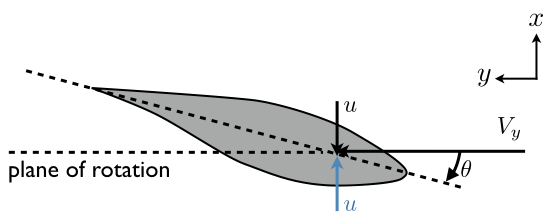
\includegraphics[width=3.5in]{figures/inflow4}
    \caption{Two possible directions for the induced axial velocity $u$.  The black $u$ is positive according to our sign convention, and the blue $u$ is negative.}
    \label{fig:inflowu}
\end{figure}

We note that we can define $W$ as (\cref{fig:inflowu}):
\begin{equation}
    W = \frac{-u}{\sin\phi} = \frac{V_y}{\cos\phi}
\end{equation}
We also cannot use the thrust coefficient directly, because we used a normalization with $V_x$ as the velocity.  We revert back to the definition of thrust in \cref{eq:beT} using the expression for $W$ above.
% \begin{equation}
% \begin{aligned}
%     T = B c_n \frac{1}{2}\rho \frac{u^2}{\sin^2 \phi} c dr\\
% \end{aligned}
% \end{equation}

From the Kutta-Joukowski theorem, the direction of $u$ and $c_n$ must be opposite.  Thus, for the case of $u > 0$ (remember a positive u is in the negative x-direction using the wind turbine convention), then $c_n$ must be positive, and $\phi < 0$.  The opposite is true for the case with $u < 0$: $c_n < 0$ and $\phi > 0$.  We can determine these signs a priori, unlike the more general case, because the velocity is strictly determined by $u$ and not $V_x - u$, and the tangential velocity has no induction.  The direction of circulation can change, depending on the sign of $V_y$, but the signs of $c_n$ and $u$ cannot.


% Similarly, for torque we use \cref{eq:beQ} and note from \cref{fig:inflowv} that
% \begin{equation}
%     W = \frac{V_x}{\sin\phi} = \frac{v}{\cos\phi}
% \end{equation}
% \begin{equation}
% \begin{aligned}
% Q = B r c_t \frac{1}{2}\rho \frac{V_y^2}{\cos^2 \phi} c dr\\
% \end{aligned}
% \end{equation}

% [TODO: move this to BEM: The inflow angle is unknown, so we ignore the downwash]
% \[Q = B r c_t \frac{1}{2}\rho V_y^2 c dr\]

If $V_y = 0$, then from the Kutta-Joukowski theorem, $a = 0$.  Also, $a^\prime$ is undefined, because of the normalization by $V_y$ and so we must refer to the total tangential induced velocity $v$.  There are two possibilities for $v$ shown in black and blue in \cref{fig:inflowv}.  From the Kutta-Joukowski theorem we know that $c_t$ and $v$ must have opposite signs.  We will consider $v$ as positive in the direction of a positive $a^\prime$ (for a positive $V_y$), thus the black $v$ is positive.  Two cases yield the following possibilities for $V_x > 0$ (with similar results for $V_x < 0$): either $\phi \in (0, \pi/2)$, in which case $c_t > 0$ and $v > 0$ or $\phi \in (\pi/2, \pi)$, in which case $c_t < 0$ and $v < 0$.

In either case we can define thrust and torque using \cref{eq:beT,eq:beQ} where from \cref{fig:inflowv} we see that
\begin{equation}
    W = \frac{V_x}{\sin\phi} = \frac{v}{\cos\phi}
\end{equation}


\begin{figure}[htbp]
\centering
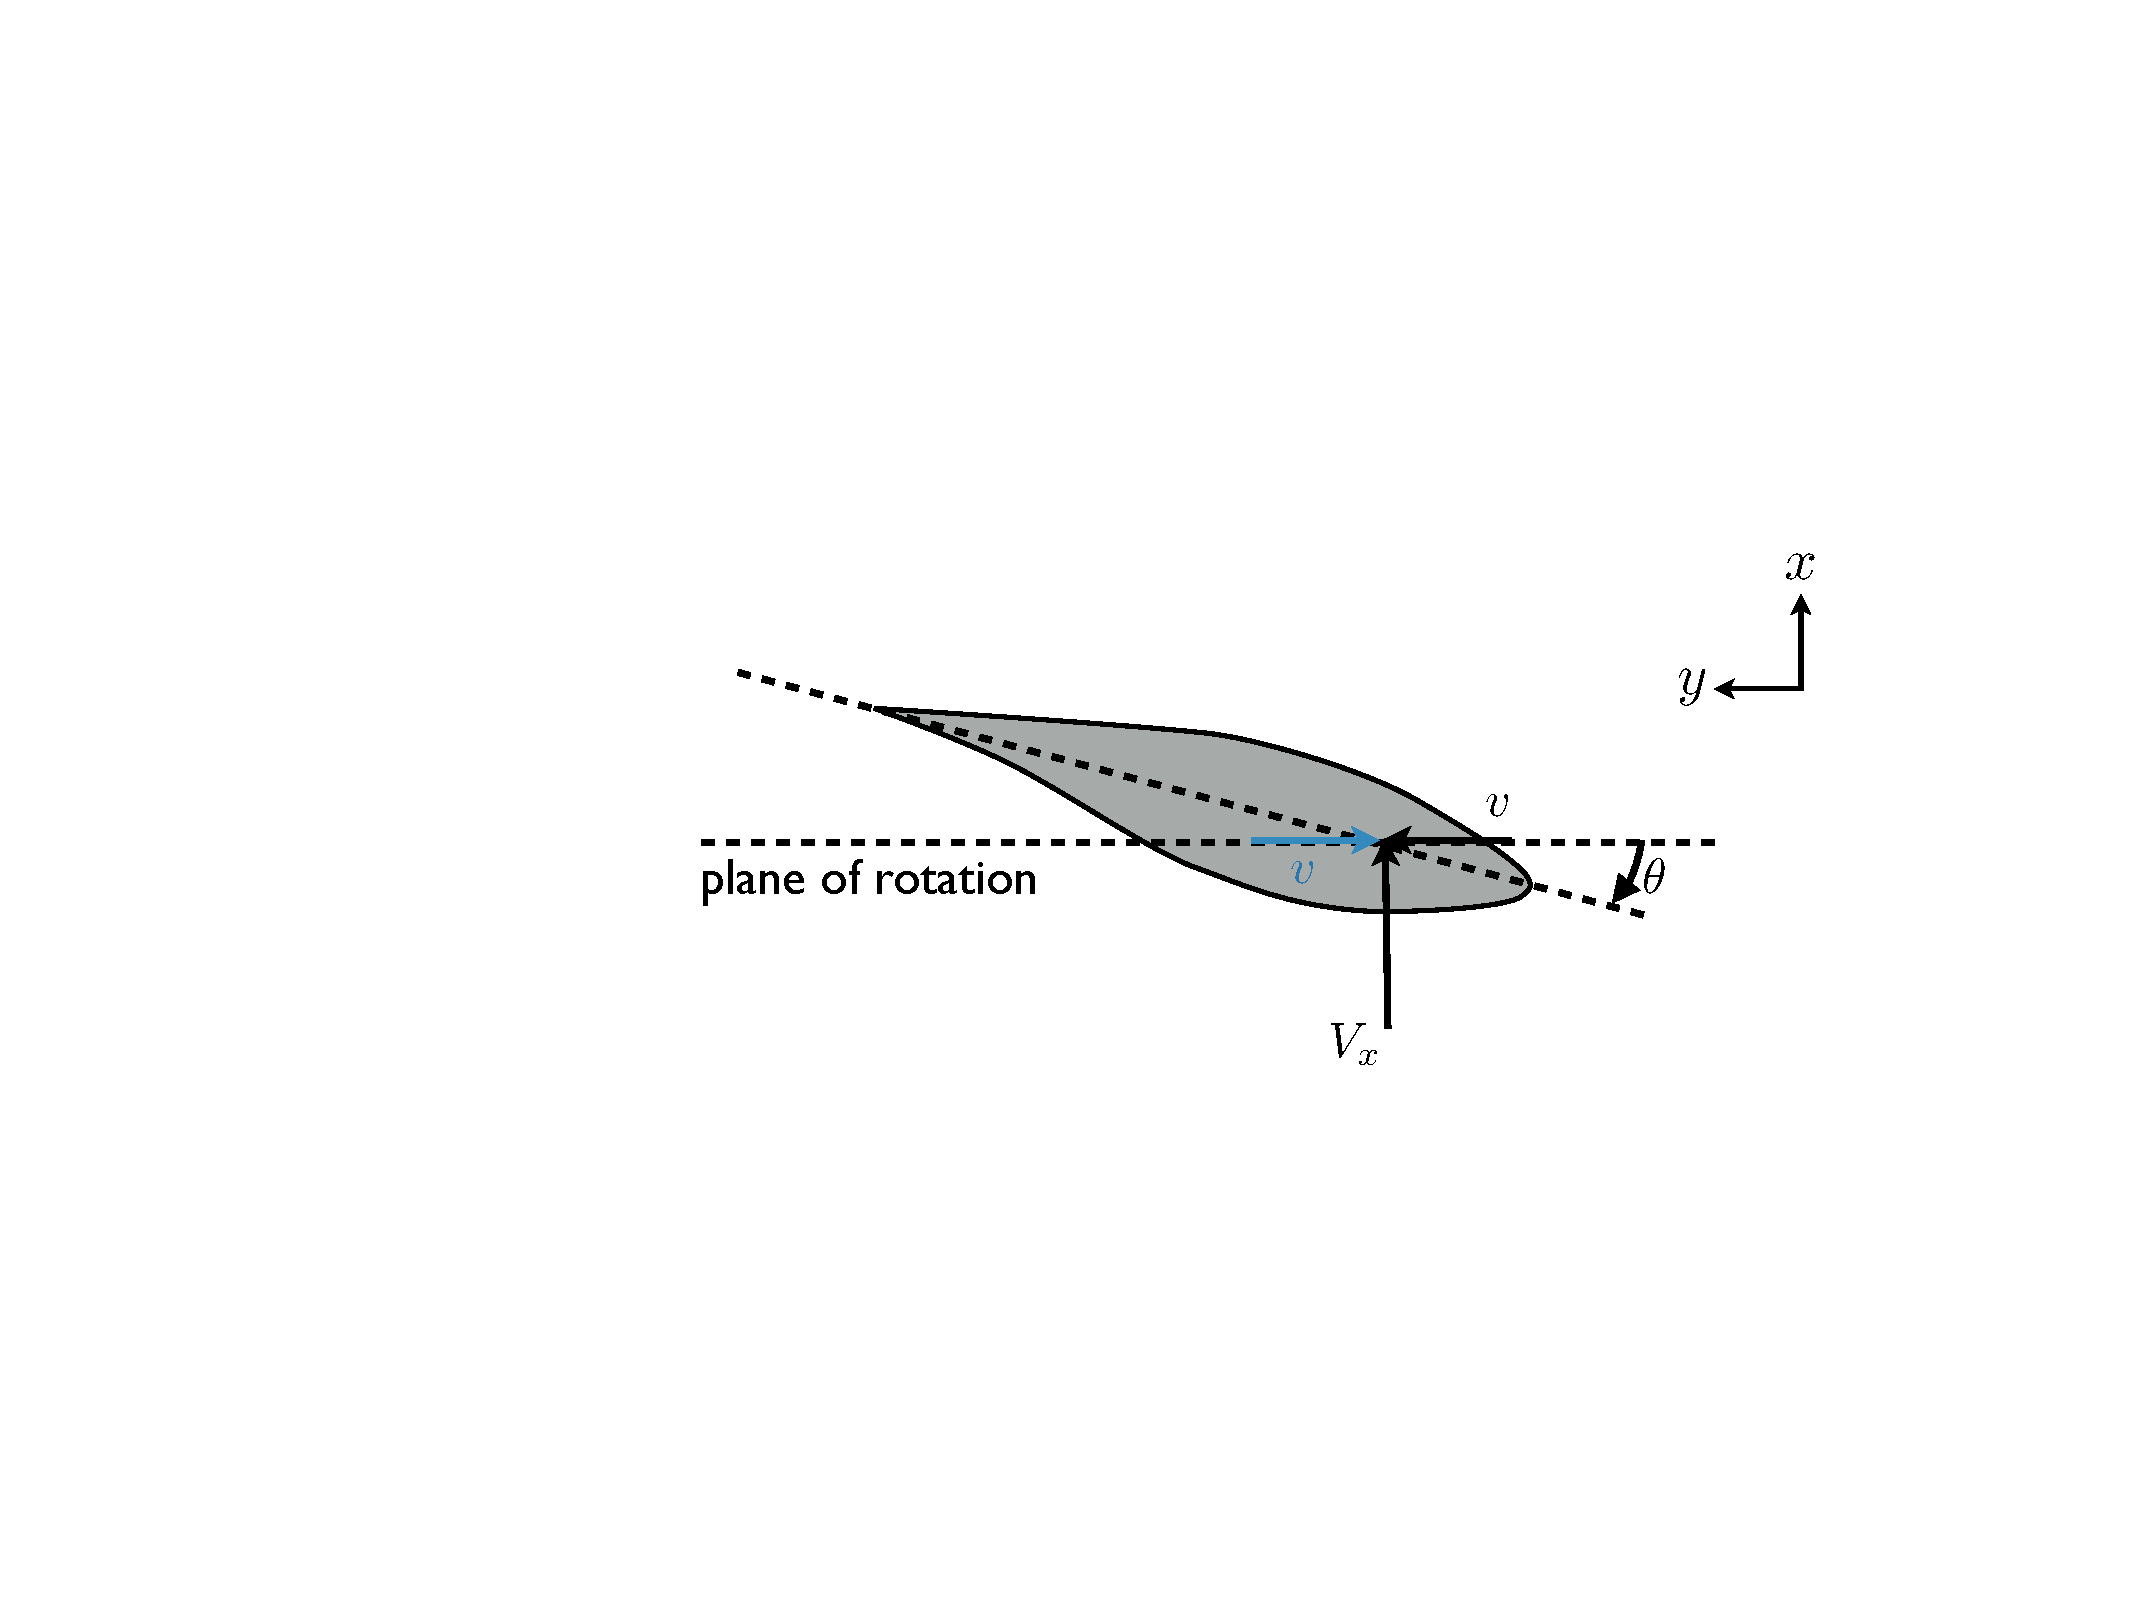
\includegraphics[width=3.5in]{figures/inflow5}
\caption{}
\label{fig:inflowv}
\end{figure}

\subsubsection{Propellers}

Conventionally, the inflow for a propeller looks like that shown in \cref{fig:inflowprop}.  To reuse the current derivation, we must use consistent inputs.  The positive directions for $a$, $a^\prime$, $\phi$, $\theta$ and $V_x$ are all opposite that of the above derivation.  Most of these will be accounted for automatically, as already discussed.  If we continue to define the total velocity as $V_x (1 - a)$, for example, then a negative value of $a$ corresponds to propeller operation.  Similarly, for $a^\prime$.  We will also use the same definition of $\phi$, so the $\phi$ pictured in \cref{fig:inflowprop} would be a negative value.

Two changes explicit changes must be made, because the they are user inputs.   The positive direction for $V_x$ and $\theta$ are defined as positive in the opposite direction of what we have been using.  This is remedied by internally switching the sign for $V_x$ and $\theta$ after they have been supplied by the user.  With this change, no others changes are required.  We can see, for example, that the angle of attack is correctly computed with consistent definitions (using a negative sign for $\theta$ and $\phi$):
\begin{equation}
    \begin{aligned}
        -\theta = -\phi + \alpha\\
        \alpha = \phi - \theta\\
    \end{aligned}
\end{equation}
This is the same definition for the angle of attack defined in \cref{eq:aoa}.

For the outputs a few explicit changes are made as well.  The induced velocity u sign changes because of the sign change on $V_x$.  We also change the definition for the tangential force, because a propeller defines a positive tangential force in the opposite direction to that of a turbine.  
% Similarly, we change the sign on the induced velocity v to correspond to the normal convention of in the direction of rotation.

% [TODO: double check this. also refer to turbine-to-prop document]

\begin{figure}[htbp]
\centering
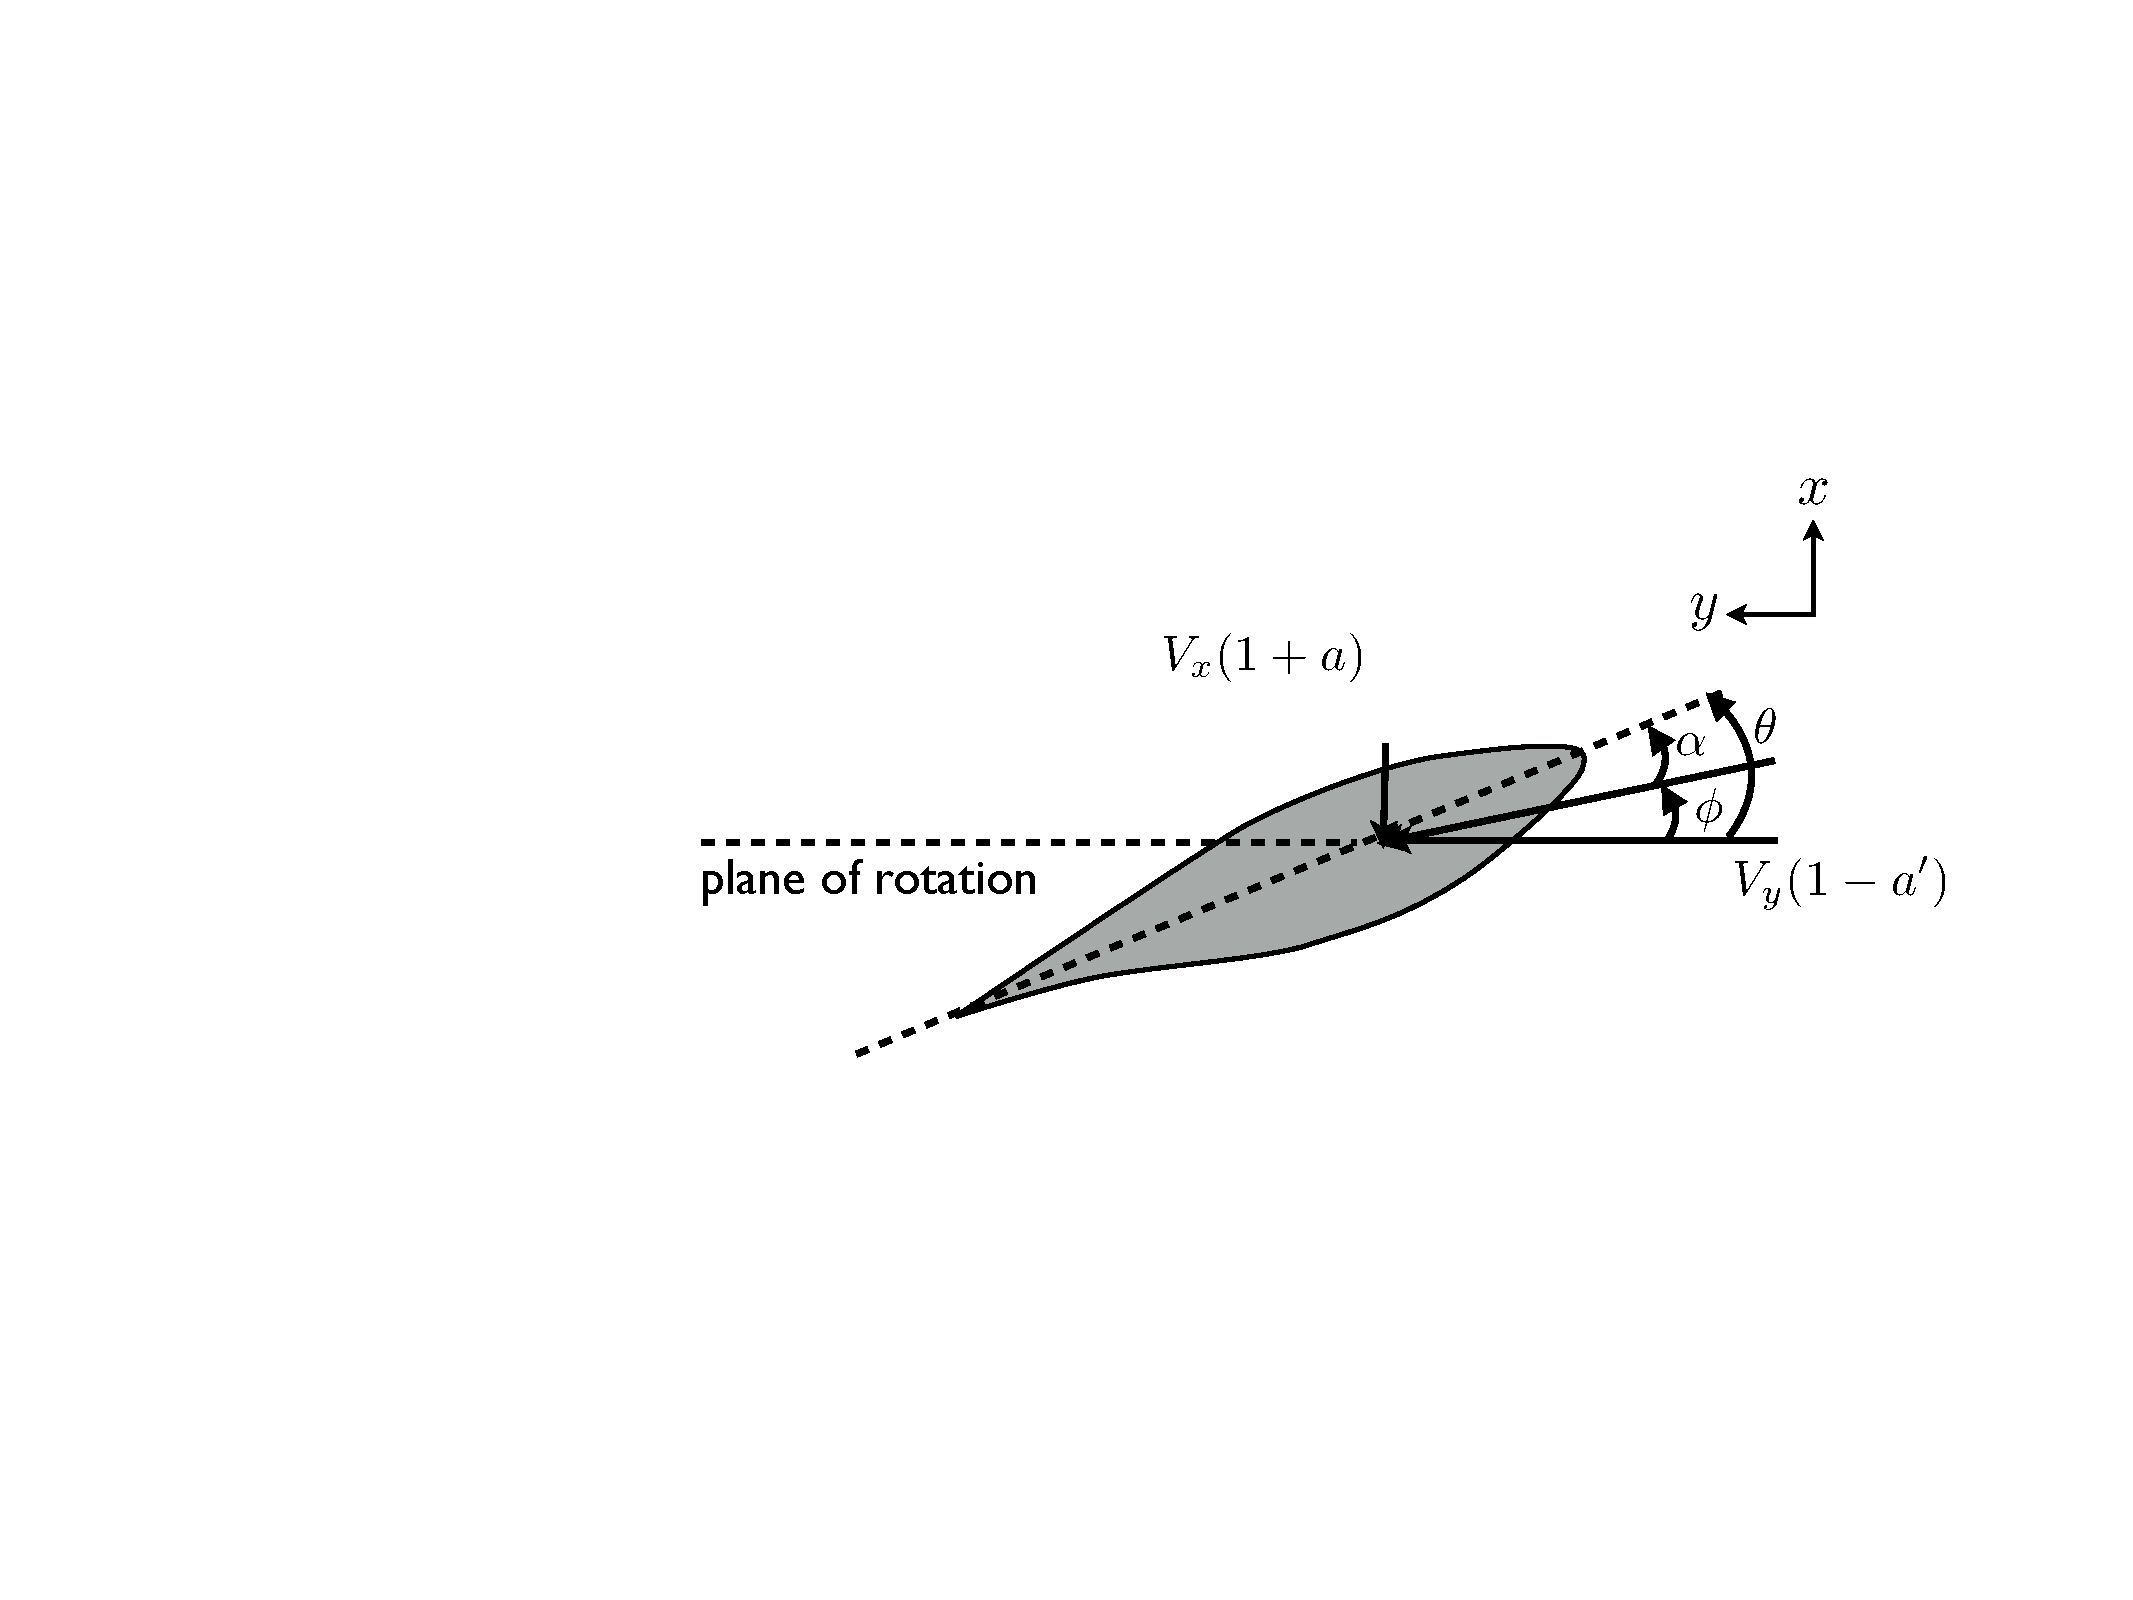
\includegraphics[width=3.5in]{figures/inflowprop}
\caption{}
\label{fig:inflowprop}
\end{figure}

\subsection{Summary}

If $V_x \ne 0, V_y \ne 0$ then
\begin{equation}
\begin{aligned}
C_T &= c_n \sigma^\prime \left(\frac{1-a}{\sin\phi}\right)^2 \\
C_Q &= c_t \sigma^\prime \left(\frac{1 + a^\prime}{\cos\phi}\right)\left(\frac{1 - a}{\sin\phi}\right)\left(\frac{V_y}{V_x}\right)\\
\end{aligned}
\end{equation}
Otherwise, use
\begin{equation}
\begin{aligned}
    T &= B c_n \frac{1}{2}\rho W^2 c dr \\
    Q &= B r c_t \frac{1}{2}\rho W^2 c dr \\
\end{aligned}
\end{equation}
where
\begin{equation}
    W =
    \begin{cases}
        \frac{-u}{\sin\phi} = \frac{V_y}{\cos\phi} & V_x = 0
        \begin{cases}
            V_y > 0, u < 0, \phi \in (0, \pi/2), c_n < 0\\
            V_y > 0, u > 0, \phi \in (-\pi/2, 0), c_n > 0\\
            V_y < 0, u < 0, \phi \in (\pi/2, \pi), c_n < 0\\
            V_y < 0, u > 0, \phi \in (-\pi, -\pi/2), c_n > 0\\
        \end{cases}\\
        \frac{V_x}{\sin\phi} = \frac{v}{\cos\phi} & V_y = 0
        \begin{cases}
            V_x > 0, v > 0, \phi \in (0, \pi/2), c_t > 0\\
            V_x > 0, v < 0, \phi \in (\pi/2, \pi), c_t < 0\\
            V_x < 0, v > 0, \phi \in (-\pi/2, 0), c_t > 0\\
            V_x < 0, v < 0, \phi \in (-\pi, \pi/2), c_t < 0\\
        \end{cases}\\
    \end{cases}
    \label{eq:Wopt}
\end{equation}




\section{Blade Element Momentum}

We can now combine the results from momentum theory and blade element theory.  We first the linear momentum equations (thrust), and next the angular momentum equations (torque).  Finally, we discuss the residual equation which determines whether or not we have consistency between the momentum and blade element theories.

\subsection{Axial Inflow}

We equate the thrust coefficients from momentum theory and blade element theory.  For now, we consider the typical cases where $V_x \ne 0$ and $V_y \ne 0$.  The thrust coefficient from blade element theory is always the same, but the momentum thrust coefficient changes depending on the sign of $V_x$ and $a$ (\cref{eq:CTmomsum}).  There are multiple cases that must be considered depending on the sign of $V_x$ and the magnitude of $a$.

\begin{itemize}

\item Case I: $V_x > 0$ and $a \le 0.4$

Equate the corresponding thrust from momentum theory \cref{eq:CTmomsum} with that of blade element theory \cref{eq:CTbe}:
\begin{equation}
    \begin{aligned}
        4 a (1 - a) F &= c_n \sigma^\prime \left(\frac{1-a}{\sin\phi}\right)^2\\
        4 a F &= c_n \sigma^\prime \frac{(1-a)}{\sin^2\phi}\\
    \end{aligned}
\end{equation}
We now define a new nondimensional quantity for convenience:
\begin{equation}
    \kappa = \frac{c_n \sigma^\prime}{4 F \sin^2 \phi}
\end{equation}
Making this substitution, we can derive a simple expression for $a$:
\begin{equation}
    \begin{aligned}
        a &= \kappa (1-a)\\
        a &= \kappa - \kappa a\\
        a (1 + \kappa) &= \kappa\\
        a &= \frac{\kappa}{\kappa + 1}\\
    \end{aligned}
\end{equation}

The criteria for this equation was expressed in terms of $V_x > 0$ and $a \le 0.4$.  However, a criteria in terms of $a$ is not convenient, because that is the quantity we are solving for.  Instead, we will express the criteria in terms of $\kappa$, which is known beforehand.  Additionally, rather than using $V_x$ to distinguish the cases, we will transform the criteria in terms of $\phi$.  As we will see later, this will allow for consolidation of the various cases.

First, just from inspection of \cref{fig:inflow2} we see that if $V_x > 0$ and $a \le 0.4$ we must have $\phi > 0$.  Next, this equation only applies if $a \le 0.4$ or in other words:
\begin{equation}
    \begin{aligned}
        \frac{\kappa}{\kappa + 1} &\le 0.4\\
        \kappa &\le 0.4 (\kappa + 1) ,\quad \text{ (assuming $\kappa + 1 > 0$ or in other words $\kappa > -1$)}\\
        0.6 \kappa &\le 0.4 \\
        \kappa &\le \frac{2}{3} \\
    \end{aligned}
\end{equation}
Thus, this equation applies if $-1 < \kappa \le 2/3$.

\item Case II: $V_x < 0$ and $a \le 0.4$

Equate the thrust from momentum theory \cref{eq:CTmomsum} and blade element theory \cref{eq:CTbe} yields:
\begin{equation}
    - 4 a (1 - a) F = c_n \sigma^\prime \left(\frac{1-a}{\sin\phi}\right)^2
\end{equation}
This is identical to case I, except we must replace $\kappa$ with $-\kappa$:
\begin{equation}
    a = \frac{\kappa}{\kappa - 1}
\end{equation}

From inspection of \cref{fig:inflow2} we see that if $V_x < 0$ and $a \le 0.4$ we must have $\phi < 0$.  Next, the conditions for $\kappa$ also must be multiplied by $-1$.  Thus, this equation applies if $-2/3 \le \kappa < 1$.  In short, we can use Case I exactly, if we replace $\kappa$ with $-\kappa$.


\item Case III: $V_x > 0$ and $a \ge 1$

This case yields:
\begin{equation}
    - 4 a (1 - a) F = c_n \sigma^\prime \left(\frac{1-a}{\sin\phi}\right)^2
\end{equation}
which results in the same formula as Case II:
\begin{equation}
    a = \frac{\kappa}{\kappa - 1}
\end{equation}

The condition for $\phi$ (see \cref{fig:inflow2}) is $\phi < 0$.  The condition for $\kappa$ is:
\begin{equation}
    \begin{aligned}
        a &\ge 1\\
        \frac{\kappa}{\kappa -1} &\ge 1\\
        \kappa &\ge \kappa -1,\quad \text{ (assuming $\kappa - 1 > 0$ or in other words $\kappa > 1$)} \\
        0 &\ge -1,\quad \text{this is always true, assuming the above condition}
    \end{aligned}
\end{equation}
Thus, we require $\kappa > 1$.

\item Case IV: $V_x < 0$ and $a \ge 1$

This case yields:
\begin{equation}
    4 a (1 - a) F = c_n \sigma^\prime \left(\frac{1-a}{\sin\phi}\right)^2
\end{equation}
which results in the same formula as Case I:
\begin{equation}
    a = \frac{\kappa}{\kappa + 1}
\end{equation}

The condition for $\phi$ (see \cref{fig:inflow2}) is $\phi > 0$.  The condition for $\kappa$ is:
\begin{equation}
    \begin{aligned}
        a &\ge 1\\
        \frac{\kappa}{\kappa + 1} &\ge 1\\
        \kappa &\le \kappa + 1,\quad \text{ (assuming $\kappa + 1 < 0$ or in other words $\kappa < -1$)} \\
        0 &\le 1,\quad \text{this is always true, assuming the above condition}
    \end{aligned}
\end{equation}
Thus, we require $\kappa < -1$.

\item Case V: $V_x > 0$ and $0.4 < a < 1$
\begin{equation}
\begin{aligned}
\left(\frac{50}{9} - 4F\right) a^2 - \left(\frac{40}{9} - 4F\right) a + \frac{8}{9} = c_n \sigma^\prime \left(\frac{1-a}{\sin\phi}\right)^2
\end{aligned}
\end{equation}
This yields a quadratic formula that can be solved for $a$.  After simplification it yields (noting that only the negative sign in the quadratic formula is physically possible):
\begin{equation}
a = \frac{\gamma_1 - \sqrt{\gamma_2}}{\gamma_3}
\label{eq:aemp}
\end{equation}
where
\begin{equation}
\gamma_1 = 2F\kappa - \left(\frac{10}{9} - F\right)\!, \quad \gamma_2 = 2F\kappa - F\left(\frac{4}{3} - F\right)\!,\quad
\gamma_3 = 2F\kappa - \left(\frac{25}{9} - 2F\right)
\label{eq:gamma}
\end{equation}
If the denominator in \cref{eq:aemp} is exactly zero (i.e., $\gamma_3 = 0$), then the numerator is also exactly zero.  However, the expression can still be evaluated using L'H\^{o}pital's rule and can be shown to be equal to
\begin{equation}
    a \xrightarrow{\gamma_3 \to 0} 1 - \frac{1}{2\sqrt{\gamma_2}}
    \label{eq:aconverge}
\end{equation}

From \cref{fig:inflow2} we see that $\phi > 0$ for our conditions on $V_x$ and $a$.  This expression will always yield an $a < 1$ so the limit we are concerned with is $a > 0.4$.  We can show that this occurs for $\kappa > 2/3$, which should make sense as this region was designed to connect at the border of the momentum region.


\item Case VI: $V_x < 0$ and $0.4 < a < 1$

This is identical to case V except for the negative sign in the thrust from momentum theory.  The effect is that we can repeat case V identically, but need to replace $\kappa$ with $-\kappa$.  Thus limit on $\phi$ changes to $\phi < 0$ and the limit on $\kappa$ to $\kappa < -2/3$.

\end{itemize}

Fortunately, these various cases can be consolidated.  First let's write them out:
\begin{equation}
    a =
    \begin{cases}
        \frac{\kappa}{\kappa + 1} & I: \phi > 0 \text{ and } -1 < \kappa \le 2/3 \\
        \frac{\kappa}{\kappa - 1} & II: \phi < 0 \text{ and } -2/3 \le \kappa < 1 \\
        \frac{\kappa}{\kappa - 1} & III: \phi < 0 \text{ and } \kappa > 1 \\
        \frac{\kappa}{\kappa + 1} & IV: \phi > 0 \text{ and } \kappa < -1 \\
        \frac{\gamma_1(\kappa) - \sqrt{\gamma_2(\kappa)}}{\gamma_3(\kappa)} & V: \phi > 0 \text{ and } \kappa > 2/3 \\
        \frac{\gamma_1(-\kappa) - \sqrt{\gamma_2(-\kappa)}}{\gamma_3(-\kappa)} & VI: \phi < 0 \text{ and } \kappa < -2/3 \\
    \end{cases}
\end{equation}

We see that we can immediately combine cases I and IV as well as II and III, as they use the same expression over contiguous ranges, excepting a point singularity.

\begin{equation}
    a =
    \begin{cases}
        \frac{\kappa}{\kappa + 1} & \phi > 0, \kappa \le 2/3 \text{ for } \kappa \ne -1\\
        \frac{\kappa}{\kappa - 1} & \phi < 0, \kappa \ge -2/3 \text{ for } \kappa \ne 1\\
        \frac{\gamma_1(\kappa) - \sqrt{\gamma_2(\kappa)}}{\gamma_3(\kappa)} & \phi > 0 \text{ and } \kappa > 2/3 \\
        \frac{\gamma_1(-\kappa) - \sqrt{\gamma_2(-\kappa)}}{\gamma_3(-\kappa)} & \phi < 0 \text{ and } \kappa < -2/3 \\
    \end{cases}
    \label{eq:asing}
\end{equation}
This expression can be further consolidated with the logic shown in the first half of \cref{alg:aap}.


We note the existence of a singularity at $\kappa = -1$ for $\phi > 0$ and at $\kappa = 1$ for $\phi < 0$.  We will see later what cases this condition corresponds to.

TODO: move somewhere else.  That condition can be handled separately, but in the above formulation we know that $\kappa$ cannot equal -1 so we can simply check that condition and return a nonzero residual

\subsection{Tangential Inflow}

We now equate the torque from blade element theory (\cref{eq:CQbe}) with the torque from momentum theory (\cref{eq:CQmom}).  Again, for now we focus on the typical cases where $V_x \ne 0$ and $V_y \ne 0$.

There are two cases.  First, $V_x > 0$:
\begin{equation}
\begin{aligned}
 c_t \sigma^\prime \left(\frac{1 + a^\prime}{\cos\phi}\right)\left(\frac{1 - a}{\sin\phi}\right)\frac{V_y}{V_x} &= 4 F a^\prime (1 - a) \frac{V_y}{V_x}\\
 c_t \sigma^\prime \left(\frac{1 + a^\prime}{\cos\phi\sin\phi}\right)&= 4 F a^\prime \\
\end{aligned}
\end{equation}
Similar to the axial induction derivation, we define a new nondimensional quantity for convenience:
\begin{equation}
    \kappa^\prime = \frac{c_t \sigma^\prime}{4 F \sin\phi \cos\phi}
\end{equation}
With that substitution we can solve for $a^\prime$ as
\begin{equation}
    a^\prime = \frac{\kappa^\prime}{1 - \kappa^\prime}
    \label{eq:aprime}
\end{equation}
Note that this is defined everywhere except when $\kappa^\prime = 1$ (we will see later where the $V_x > 0, \kappa^\prime = 1$ case corresponds to).

Similarly, for $V_x < 0$ we obtain
\begin{equation}
    a^\prime = \frac{-\kappa^\prime}{1 + \kappa^\prime}
\end{equation}
Or equivalently, we can use the same formula in \cref{eq:aprime}, but negate $\kappa^\prime$ if $V_x < 0$.  We see that the $V_x < 0$ case is defined everywhere except when $\kappa^\prime = -1$.  These two cases can be combined into the algorithm shown in the bottom half of \cref{alg:aap}.





\subsection{Residual Equation}

With the induction factors calculated the residual function can be computed. This residual equation ensures compatibility between the momentum theory, and blade element theory. The current induction factors may not be correct, as they depend on the angle of attack, which in turn depends on the induction factors themselves.  Thus, an iterative, or root-finding methods is necessary.

Conventionally, this is solved by considering $a$ and $a^\prime$ as the unknowns and solving using a two-dimensional root finding approach \cite{Manwell2009-Wind-Energy,Hansen2008-Aerodynamics-Wind,Burton2011-Wind-Energy}.  However, this can be solved much more effectively by examining \cref{fig:inflow2} and realizing that we can define the velocity vectors equivalently by considering the two unknowns to be $W$ and $\phi$ \cite{Ning2014-Simple-Solution}.  This results in a big simplification because $W$ only appears in the Reynolds number, and as discussed in \cref{sec:be} we can almost always safely neglect the induction factors in the Reynolds number calculation (or if we really want to include them this can be done easily in an extra iteration). In other words, we can reduce our unknowns to one: $\phi$.  This has the massive advantage that one-dimensional root finding problems are easier to solve, and unlike two-dimensional ones, we can guarantee convergence as long as we can find a suitable bracket.

The residual function is taken from \cref{fig:inflow2} where we see that
\[\tan\phi = \frac{V_x (1 - a)}{V_y (1 + a^\prime)}\]
This equation can be arranged many different ways to form a residual function, but not all will lead to a reliably convergent method. Singularities in the residual function are unavoidable, but it is convenient to have the quantities $(1 - a)$ and $(1 + a^\prime)$ in the denominator so that singularities occur at the predefined locations: $\phi = 0, \pm\pi$ \cite{Ning2014-Simple-Solution}. These locations are particularly convenient because they also separate regions where the physics change.  We rearrange in the residual form below:
\begin{equation}
    \mathcal{R}(\phi) = \frac{\sin\phi}{(1 - a(\phi))} - \frac{V_x}{V_y} \frac{\cos\phi}{(1 + a^\prime(\phi))} = 0
    \label{eq:residual}
\end{equation}

This one-dimensional equation is easily solved, if we can determine a bracket.  For the conventional methodology and modes of operation ($V_x > 0$ and $V_y > 0$), the brackets can be determined a priori \cite{Ning2014-Simple-Solution}.  However, for more general conditions the brackets may need to be established numerically.  All that is needed to establish a bracket, $(\phi_L, \phi_U)$, is to find two points between which the residual function changes sign (i.e., $\mathcal{R}(\phi_L)\mathcal{R}(\phi_U) < 0$).

From the signs of $V_x$ and $V_y$, we know where a bracket is most likely to be found.  \Cref{tab:quadrants} divides the $\phi$ range into four quadrants, which are also depicted in \cref{fig:quadrants}:
\begin{table}[htb]
\centering
\caption{The use of $\epsilon$ is to avoid the singularities at $\phi = 0$ and $\phi = \pi$.}
\label{tab:quadrants}
\begin{tabular}{@{}ll@{}}
\toprule
Quadrant & $\phi$ range\\
\midrule
I & $(\epsilon, \pi/2)$ \\
II & $(-\pi/2, -\epsilon)$ \\
III & $(\pi/2, \pi-\epsilon)$ \\
IV & $(-\pi+\epsilon, -\pi/2)$ \\
\bottomrule
\end{tabular}
\end{table}
\begin{figure}[htbp]
\centering
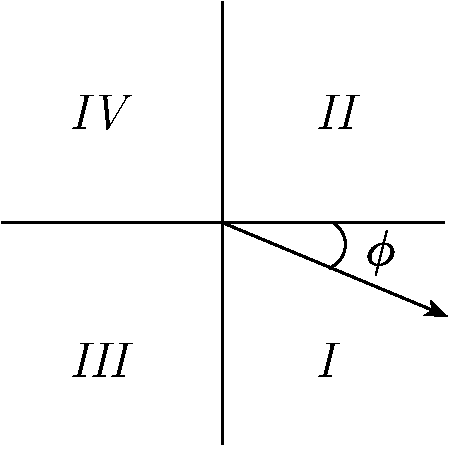
\includegraphics[width=2.5in]{figures/quadrants}
\caption{caption}
\label{fig:quadrants}
\end{figure}

We search quadrant in the order shown in \cref{tab:brackets}.  It would be very rare that the solution would not occur in the first quadrant listed, but for completeness we list all possibilities in the order of likelihood.  Within each quadrant, we still need to establish a bracket around a root.  Generally there is not more than one solution in a given quadrant.  However, the numerical possibility of multiple solutions exists and so we search for the solution closes to $\phi = 0$, as that is the most physically likely.  The method we use subdivides the quadrant into $n_{int}$ intervals, where $n_{int}$ is a user-defined parameter defaulting to 20.  Starting at the lower bound, we march forward towards the upper bound looking for a change in sign.  If this fails, one could try a finer discretization, or move to the next quadrant.

\begin{table}[htb]
\centering
\caption{}
\label{tab:brackets}
\begin{tabular}{@{}ccl@{}}
\toprule
$V_x$ & $V_y$ & quadrant order \\
\midrule
+ & + & I, II, III, IV \\
- & + & II, I, IV, III \\
+ & - & III, IV, I, II \\
- & - & IV, III, II, I \\
\bottomrule
\end{tabular}
\end{table}



\begin{algorithm}[htbp]
\caption{Solve the residual equation $\mathcal{R}(\phi)$}
\begin{algorithmic}

\If {$\phi < 0$}
    \State $\kappa = -\kappa$
\EndIf
\\
\If {$\kappa \le 2/3$}
    \State $a = \frac{\kappa}{\kappa + 1}$
    \Comment{if $\kappa = -1$ return any nonzero residual.}
\Else
    \State $a = \frac{\gamma_1 - \sqrt{\gamma_2}}{\gamma_3}$
    \Comment{if $\gamma_3 = 0$ use \cref{eq:aconverge}.}
\EndIf
\\
\If {$V_x < 0$}
    \State $\kappa^\prime = -\kappa^\prime$
\EndIf
\\
\State $a^\prime = \kappa^\prime/(1 - \kappa^\prime)$
\Comment{if $\kappa^\prime = 1$ return any nonzero residual.}
\\
\State $\mathcal{R}(\phi) = \frac{\sin\phi}{(1 - a(\phi))} - \frac{V_x}{V_y} \frac{\cos\phi}{(1 + a^\prime(\phi))}$
\end{algorithmic}
\label{alg:aap}
\end{algorithm}

\subsection{No Wind In One of the Directions}

The cases where no wind exists in one of the directions (i.e., $V_x = 0$ or $V_y = 0$) must be treated separately as the solution approach cannot be combined with the normal cases.

\subsubsection{No Wind in the x-direction}
If $V_x = 0$, equating thrust from the momentum and blade element theories and simplifying yields for $u > 0$:
\begin{equation}
\begin{aligned}
    4 \pi r \rho u^2 F dr &= B c_n \frac{1}{2} \rho W^2 c dr\\
    4 u^2 F&= \sigma^\prime c_n W^2\\
\end{aligned}
\end{equation}
The value for $W$ is shown in \cref{eq:Wopt} for $V_x = 0$.  Let's first use the first option: $W = -u/\sin\phi$.  Substituting into the above expression and simplifying yields
\begin{equation}
\kappa = 1
\end{equation}
Conversely, if $u < 0$ the same expression yields
\begin{equation}
\kappa = -1
\end{equation}
We note that the first case with $u > 0$ implies that $\phi < 0$ (see velocity  triangle in \cref{fig:inflowu}) and results in the expression $\kappa = 1$.  This case fills in our singularity noted in \cref{eq:asing}.  In other words, the case $\phi < 0, \kappa = 1$, only exists for $V_x = 0$.  Similarly, the derivation for $u < 0$ corresponds to $\phi > 0$ with the result that $\kappa = -1$, which fills in the other singularity.  Thus, the previous formulation ($V_x \ne 0, V_y \ne 0$) should ignore the case $\kappa = -1$ as it won't satisfy the residual equation.  Any nonzero residual could be returned.  We deal with this case explicitly in this section with a different formulation.

While, the substitution $W = -u/\sin\phi$ led to the insight of filling in our singularity, it doesn't help us solve the equation.  Instead, we will use the second substitution from \cref{eq:Wopt}: $W = V_y / \cos\phi$ (incidentally, one of each of the W expressions could be used instead, either approach will lead to the same solution once the residual is converged).  This substitutions leads to (for the case $u > 0$, which corresponds to $\phi < 0$):
\begin{equation}
\begin{aligned}
4 u^2 F&= \sigma^\prime c_n \frac{V_y^2}{\cos^2\phi}\\
u&= \sqrt{\frac{\sigma^\prime c_n V_y^2}{4 F \cos^2\phi}}\\
\end{aligned}
\end{equation}
Conversely if $u < 0$ then the sign on the momentum portion of thrust switches and we have:
\begin{equation}
\begin{aligned}
- 4 u^2 F&= \sigma^\prime c_n \frac{V_y^2}{\cos^2\phi}\\
u&= -\sqrt{\frac{-\sigma^\prime c_n V_y^2}{4 F \cos^2\phi}}\\
\end{aligned}
\end{equation}
where the minus sign in the front of the sqrt arises because the sqrt could have either sign, but we know that $u < 0$ for this case.  We see that these expression are consistent with the conditions derived in \cref{eq:Wopt}.  Namely, those conditions require that if $u > 0$ then $c_n > 0$ and if $u < 0$ then $c_n < 0$.  The argument under the sqrt follows the sign of $c_n$ (all other entires are positive), and so these conditions lead to positive sqrt arguments, as is physically consistent.  Thus, if during a residual solve a $c_n$ is computed inconsistent with these cases we can skip evaluating the sqrt and return any nonzero residual.

% If on the other hand, $V_y < 0$

%
% For $V_x = 0, u > 0$, we have two possibilities depending on the sign of $V_y$.  If $V_y > 0$ then
%
% two possibilities depending on the sign of $\phi$ (and thus the appropriate sign of $u$ and $c_n$):
% If $\phi > 0$ then $c_n < 0$ and $u < 0$ from blade element theory:
% \begin{equation}
% \begin{aligned}
%     - 4 \pi r \rho u^2 F dr &= B c_n \frac{1}{2} \rho \frac{u^2}{\sin^2\phi} c dr\\
%     \kappa = -1 \\
% \end{aligned}
% \end{equation}
% Conversely, if $\phi < 0$ then $c_n > 0$ and $u > 0$ from blade element theory:
% \begin{equation}
% \begin{aligned}
%     4 \pi r \rho u^2 F dr &= B c_n \frac{1}{2} \rho \frac{u^2}{\sin^2\phi} c dr\\
%     \kappa = 1 \\
% \end{aligned}
% \end{equation}
% Incidentally, these cases fills in the missing singularities in \cref{eq:??} where we had missing singularities for $\phi > 0, \kappa = -1$, and $\phi < 0, \kappa = 1$.  We see now that the cases corresponds to when $V_x = 0$.
%
% Unfortunately, this way of expressing the equations doesn't permit a solution for $\phi$.  Instead, we reexpress $W$ in the momentum equation [ref] as $W = V_y\cos\phi$.  The result for $\phi > 0$ is:
% \begin{equation}
% \begin{aligned}
%     - 4 \pi r \rho u^2 F dr &= B c_n \frac{1}{2} \rho \frac{V_y^2}{\cos^2\phi} c dr\\
%     u &= -\sqrt{\frac{-\sigma^\prime c_n V_y^2}{4 F \cos^2\phi}} \\
% \end{aligned}
% \end{equation}
% where we note, as observed in the blade element solution, that the only physically consistent solution is for $c_n < 0$.  The sign for $u$ could be positive or negative, but we know it is negative based on the discussion in blade element theory ([sec]).
%
% The result for $\phi < 0$ is:
% \begin{equation}
% \begin{aligned}
%     4 \pi r \rho u^2 F dr &= B c_n \frac{1}{2} \rho \frac{V_y^2}{\cos^2\phi} c dr\\
%     u &= \sqrt{\frac{\sigma^\prime c_n V_y^2}{4 F \cos^2\phi}} \\
% \end{aligned}
% \end{equation}
% which must have $c_n > 0$.

The residual equation can be found by using the velocity triangle in \cref{fig:inflowu} (note that a positive $u$ is in the -x direction using our convention for the positive definition of $a$) or by dividing the existing residual equation (\cref{eq:residual}) by $V_x$, noting that $u = V_x a$, then letting $V_x \rightarrow 0$.
\begin{equation}
    - \frac{\sin\phi}{u(\phi)} - \frac{\cos\phi}{V_y} = 0
\end{equation}
The relevant quadrants can be determined from the sign of $V_y$.  Because $a^\prime = 0$, just knowing the sign of $V_y$ immediately eliminates two of the four quadrants.  The sign of $u$ is not known, however knowing whether it is a propeller or a turbine (or more generally knowing the sign of the twist) gives us a good idea of what the sign of $u$ will be.  For a positive twist, the most likely scenario is $c_n < 0$ thus $u < 0$, and vice-versa for a negative twist.  The order of quadrants is defined in \cref{tab:bracket2}.

\begin{table}[htb]
\centering
\caption{$V_x = 0$, $\theta$ includes pitch}
\label{tab:bracket2}
\begin{tabular}{@{}ccl@{}}
\toprule
$V_y$ & $\theta$ & quadrant order \\
\midrule
+ & + & I, II \\
+ & - & II, I \\
- & + & III, IV \\
- & - & IV, III \\
\bottomrule
\end{tabular}
\end{table}

% Note that for this case, there is no singularity at $\phi = 0$, thus we can use different brackets.  For a turbine the most likely scenario is a negative normal force coefficient (unless the turbine has a large negative twist for some reason), thus $\phi > 0$.  Because there is no tangential induction, only one of the two quadrants is physically sensible, and this is known based on the sign of $V_y$.  The above discussion applies for a propeller but with opposite sign for $\phi$.

Once we solve this 1D equation for $\phi$, we can compute the torque distribution purely from blade element theory as momentum theory does not predict any torque for the case $V_x = 0$. We can use either expression for $W$ in \cref{eq:Wopt}.

%  to compute the thrust and torque as normal
% \begin{equation}
% \begin{aligned}
%     T^\prime = B c_n \frac{1}{2} \rho W^2 c\\
%     Q^\prime = B r c_t \frac{1}{2} \rho W^2 c\\
% \end{aligned}
% \end{equation}


\begin{algorithm}[htbp]
\caption{Solve the residual equation for the case $V_x = 0$.}
\begin{algorithmic}


\If {$\phi > 0$}
    \State $u = -\sqrt{\frac{-\sigma^\prime c_n V_y^2}{4 F \cos^2\phi}}$
    \Comment{If $c_n > 0$ return any nonzero residual}
\Else
    \State $u = \sqrt{\frac{\sigma^\prime c_n V_y^2}{4 F \cos^2\phi}}$
    \Comment{If $c_n < 0$ return any nonzero residual}
\EndIf
\\
\State $\mathcal{R}(\phi) = - \frac{\sin\phi}{u(\phi)} - \frac{\cos\phi}{V_y}$
\end{algorithmic}
\label{alg:Vx0}
\end{algorithm}

% The resulting logic is:
%
% if turbine and $V_y > 0$: search bracket $[0, \pi/2]$ (note no singularity at 0)
%
% if turbine and $V_y < 0$: search bracket $[\pi/2, \pi]$
%
% if $c_n > 0$, then return 1 or some other nonzero value for the residual.  Otherwise evaluate:
% \begin{equation}
%     u = -\sqrt{\frac{-\sigma^\prime c_n V_y^2}{4 F \cos^2\phi}}
% \end{equation}
% \begin{equation}
%     \mathcal{R}(\phi) = - \frac{\sin\phi}{u(\phi)} - \frac{\cos\phi}{V_y} = 0
% \end{equation}
%
%
% if propeller and $V_y > 0$: search bracket $[-\pi/2, 0]$ (note no singularity at 0)
%
% if propeller and $V_y < 0$: search bracket $[-\pi, -\pi/2]$
%
% if $c_n < 0$, then return 1 or some other nonzero value for the residual.  Otherwise evaluate:
% \begin{equation}
%     u = \sqrt{\frac{\sigma^\prime c_n V_y^2}{4 F \cos^2\phi}}
% \end{equation}
% \begin{equation}
%     \mathcal{R}(\phi) = - \frac{\sin\phi}{u(\phi)} - \frac{\cos\phi}{V_y} = 0
% \end{equation}

\subsubsection{No Wind in the y-direction}

If $V_y = 0$ we equate momentum theory in \cref{eq:CQmom} with blade element theory in \cref{eq:beQ}.  If $V_x > 0$ we have:
\begin{equation}
\begin{aligned}
4 \pi F r^2 v \rho V_x dr = B r c_t \frac{1}{2} \rho W^2 c dr\\
4  F v  V_x  = \sigma^\prime c_t  W^2 \\
\end{aligned}
\end{equation}
If we use one of each substitution for $W = V_x/\sin\phi$ and $W = v/\cos\phi$ from \cref{eq:Wopt} in the above expression we have
\begin{equation}
\begin{aligned}
4  F v  V_x  = \sigma^\prime c_t \frac{V_x v}{\sin\phi \cos\phi} \\
\kappa^\prime = 1\\
\end{aligned}
\end{equation}
Conversely, if we use the case $V_x < 0$, the resulting simplification is
\begin{equation}
    \kappa^\prime = -1
\end{equation}
Like the axial inflow case, these scenarios fill in the singularity shown in \cref{alg:aap}.  For the case $V_y \ne 0$, the calculation of $a^\prime$ is undefined is $\kappa^\prime = 1$ for $V_x > 0$ or if $\kappa^\prime = -1$ for $V_x < 0$.  We see now that it is undefined because that case corresponds to $V_y = 0$.  As in the axial inflow case, we simply return a nonzero residual if that case occurs in \cref{alg:aap}, and we handle the case $V_y = 0$ explicitly below.



Like before, the simplifications yielding $\kappa^\prime = \pm1$ are insightful, but don't lead to a solution process.  We can instead use either substitution for $W$, but in the following we will use $W = V_x / \sin\phi$.  This yields the following for $V_x > 0$:
\begin{equation}
    v = \frac{\sigma^\prime c_t}{4 F \sin^2\phi} V_x
\end{equation}
and if $V_x < 0$ we have
\begin{equation}
    v = -\frac{\sigma^\prime c_t}{4 F \sin^2\phi} V_x
\end{equation}
We see that $v$ follows the sign of $c_t$, which is consistent with the physics discussed in \cref{sec:nowindtan}.  We can condense these two cases as shown in \cref{alg:Vy0}.

% Solving for $v$ yields:
% \begin{equation}
%     v = \kappa^\prime V_x
%     \label{eq:vtoVx}
% \end{equation}
The residual equation is
\begin{equation}
    \frac{\sin\phi}{V_x} - \frac{\cos\phi}{v(\phi)} = 0
\end{equation}
which we can derive from the velocity triangle in \cref{fig:inflowu} or from \cref{eq:residual} where we set $V_y a^\prime = v$ then allow $V_y \rightarrow 0$.  This form of the residual is actually inconvenient because $v$ can change sign causing a singularity in the denominator.  We arrange to the mathematically equivalent, but better behaved numerically equation:
\begin{equation}
    v(\phi)\sin\phi - V_x \cos\phi = 0
\end{equation}

The quadrant search order is defined in \cref{tab:bracket3}.

Once we solve for $\phi$ we can compute the thrust and torque distributions as normal, but computing $W$ as:
\begin{equation}
    W = \frac{V_x}{\sin\phi}
\end{equation}
The algorithm for this case is shown in \cref{alg:Vy0}.

\begin{table}[htb]
\centering
\caption{$V_y = 0$, $\theta$ includes pitch}
\label{tab:bracket3}
\begin{tabular}{@{}ccl@{}}
\toprule
$V_x$ & $|\theta|$ & quadrant order \\
\midrule
+ & $< \pi/2$ & I, III \\
- & $< \pi/2$ & II, IV \\
+ & $> \pi/2$ & III, I \\
- & $> \pi/2$ & IV, II \\
\bottomrule
\end{tabular}
\end{table}

\begin{algorithm}[htbp]
\caption{Solve the residual equation for the case $V_y = 0$.}
\begin{algorithmic}
\State $v = \frac{\sigma^\prime c_t}{4 F \sin^2\phi} |V_x|$
\\
\State $\mathcal{R}(\phi) = v(\phi)\sin\phi - V_x \cos\phi$

\end{algorithmic}
\label{alg:Vy0}
\end{algorithm}

% \begin{equation}
%     T^\prime = B c_n \frac{1}{2} \rho \frac{V_x^2}{\sin^2\phi} c
% \end{equation}
% \begin{equation}
%     Q^\prime = B r c_t \frac{1}{2} \rho \frac{V_x^2}{\sin^2\phi} c
% \end{equation}

% We note substituting in \cref{eq:vtoVx} into \cref{eq:noVyresid} yields:
% \begin{equation}
%     \mathcal{R}(\phi) = \kappa^\prime(\phi) \sin\phi - \cos\phi = 0
% \end{equation}
% Thus, $V_x$ does not directly appear in the residual equation and so we don't need to worry about its sign, as is consistent with the discussion in section??.


\subsection{Inflow}

For the simplest case with uniform inflow aligned with the hub, the x- and y-components of the inflow velocity can be computed as:
\begin{equation}
\begin{aligned}
    V_x &= V_\infty \cos\Phi\\
    V_y &= \Omega r \cos\Phi
\end{aligned}
\end{equation}
and these velocities are the same at any azimuthal station.  For a more general case, we use the angle definitions shown in \cref{fig:angles} (TODO: include precone).
\begin{figure}[htbp]
\centering
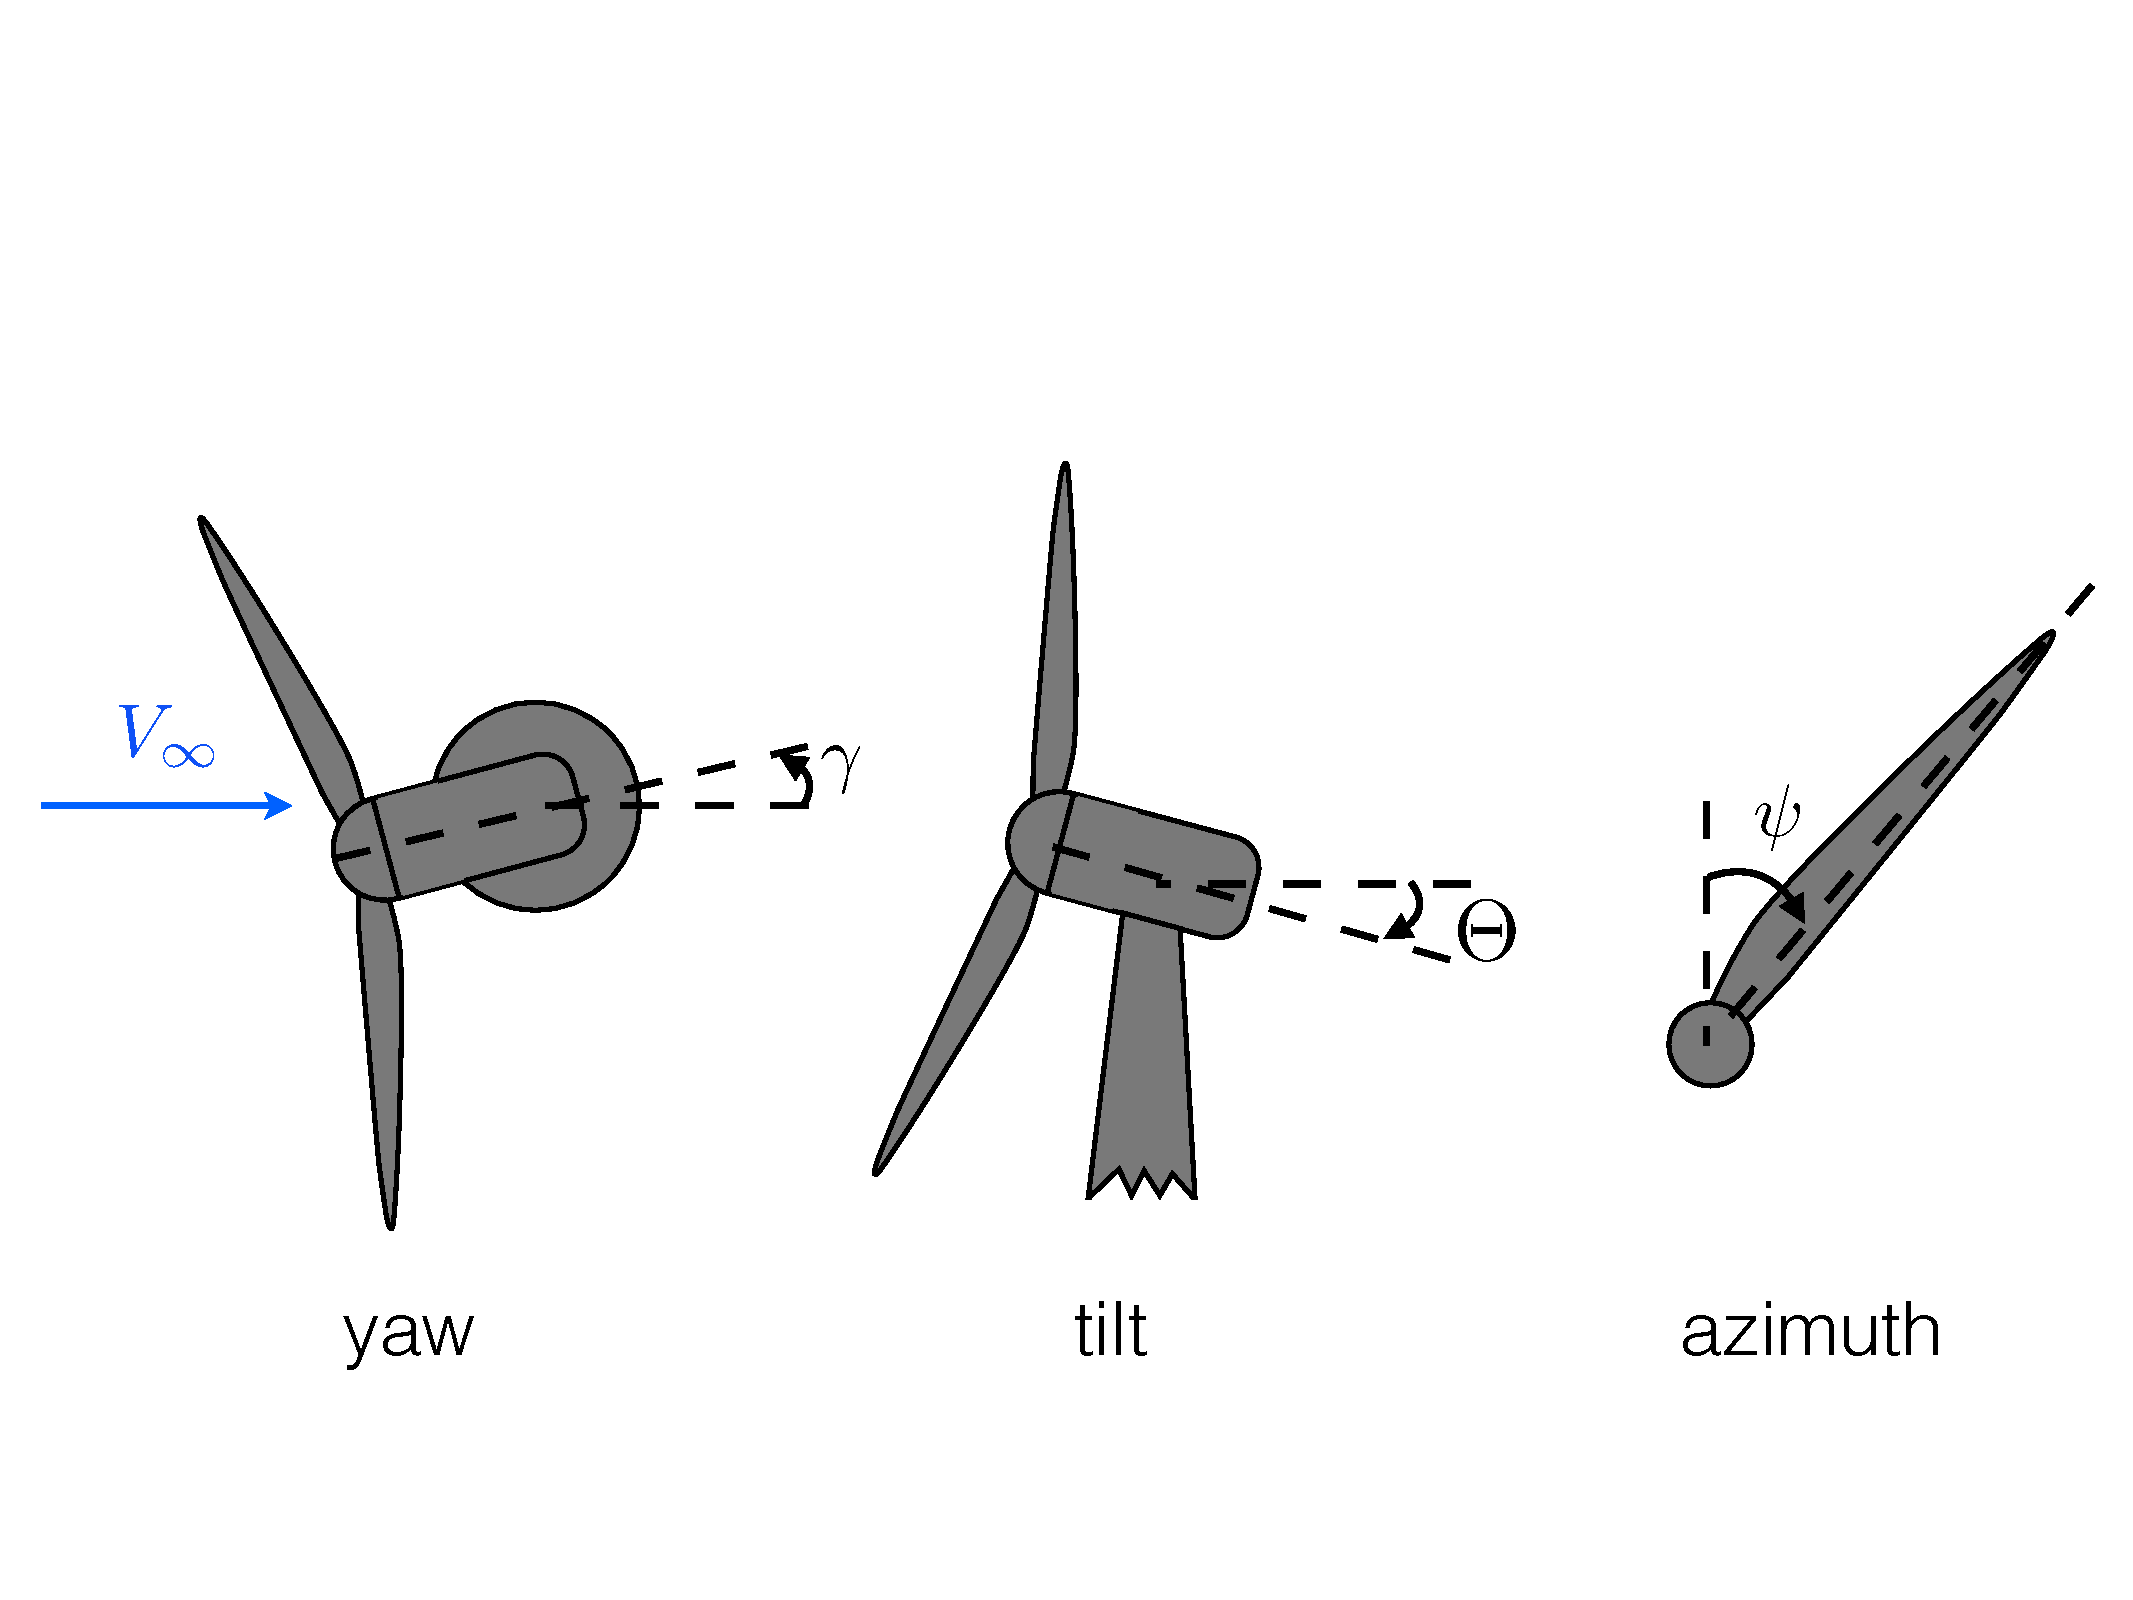
\includegraphics[width=3.5in]{figures/angles}
\caption{Definitions for some of the relevant geometric angles.}
\label{fig:angles}
\end{figure}
We also allow for wind shear across the rotor face.  To account for the velocity change across the hub face we compute the height of each blade location relative to the hub using coordinate transformations:
\begin{equation}
    z_h = r \cos\Phi \cos\psi \cos\Theta + r \sin\Phi\sin\Theta
\end{equation}
then apply the shear exponent ($\alpha$):
\begin{equation}
    V_{shear} = V_{hub} \left(1 + \frac{z_h}{H_{hub}} \right)^\alpha
\end{equation}
where $H_{hub}$ is the hub height.  Finally, we can compute the x- and y-components of velocity with additional coordinate transformations:
\begin{equation}
\begin{aligned}
V_x &= V_{shear} ((\cos \gamma \sin \Theta \cos \psi + \sin \gamma \sin \psi)\sin \Phi + \cos \gamma \cos \Theta \cos \Phi)\\
V_y &= V_{shear} (\cos \gamma \sin \Theta\sin \psi - \sin \gamma \cos \psi) + \Omega r \cos\Phi
\end{aligned}
\end{equation}

Completely general cases can be handled as well (e.g., with turbulence, blade motion, wakes), but in these cases the user must input the velocity distributions themselves rather than use these convenience methods.


\subsection{Loads}

Once the residual equation is solved, the distributed loads (force per unit length) can be computed as defined in \cref{alg:loads}.
\begin{algorithm}[htbp]
\caption{Solve for the load distributions.}
\begin{algorithmic}
\If {$V_x = 0$}
% \State $W = \frac{V_y}{\cos\phi}$
\State $W^2 = u^2 + V_y^2$
\ElsIf {$V_y = 0$}
% % \State $W = \frac{V_x}{\sin\phi}$
\State $W^2 = V_x^2 + v^2$
\Else
\State $W^2 = (V_x(1 - a))^2 + (V_y(1 + a^\prime))^2$
\EndIf
\\
\\
\State $q = \frac{1}{2}\rho W^2$
\State $N^\prime = c_n q c$
\State $T^\prime = c_t q c$

\end{algorithmic}
\label{alg:loads}
\end{algorithm}

TODO: replace with no curvature/sweep.  I don't feel like our methods are equipped to handle that anyway.

The local airfoil coordinate system is shown in \cref{fig:csys}.  The z-direction is directed along the blade, the y-direction opposite to the rotational velocity, and the x-direction given by the right-hand rule (nominally in the downwind direction).  This coordinate system is equally valid for downwind turbines, but in both cases, assumes that the rotor is rotating clockwise when viewed from upwind.  Because the blade may be curved (whether due to a nonstraight design or deflection), the coordinate system is local to each section along the blade (\cref{fig:curved}).  Swept blades can also be handled, but it is assumed that sweep is accomplished through shearing, rather than rotation, so that the local airfoils and local coordinate systems are still defined relative to the unswept rotation direction (\cref{fig:swept}).

\begin{figure}[htbp]
\centering
 \subfloat[Side view of curved blade.  Coordinate system is normal to curvature.]{
   \makebox[3.0in][c]{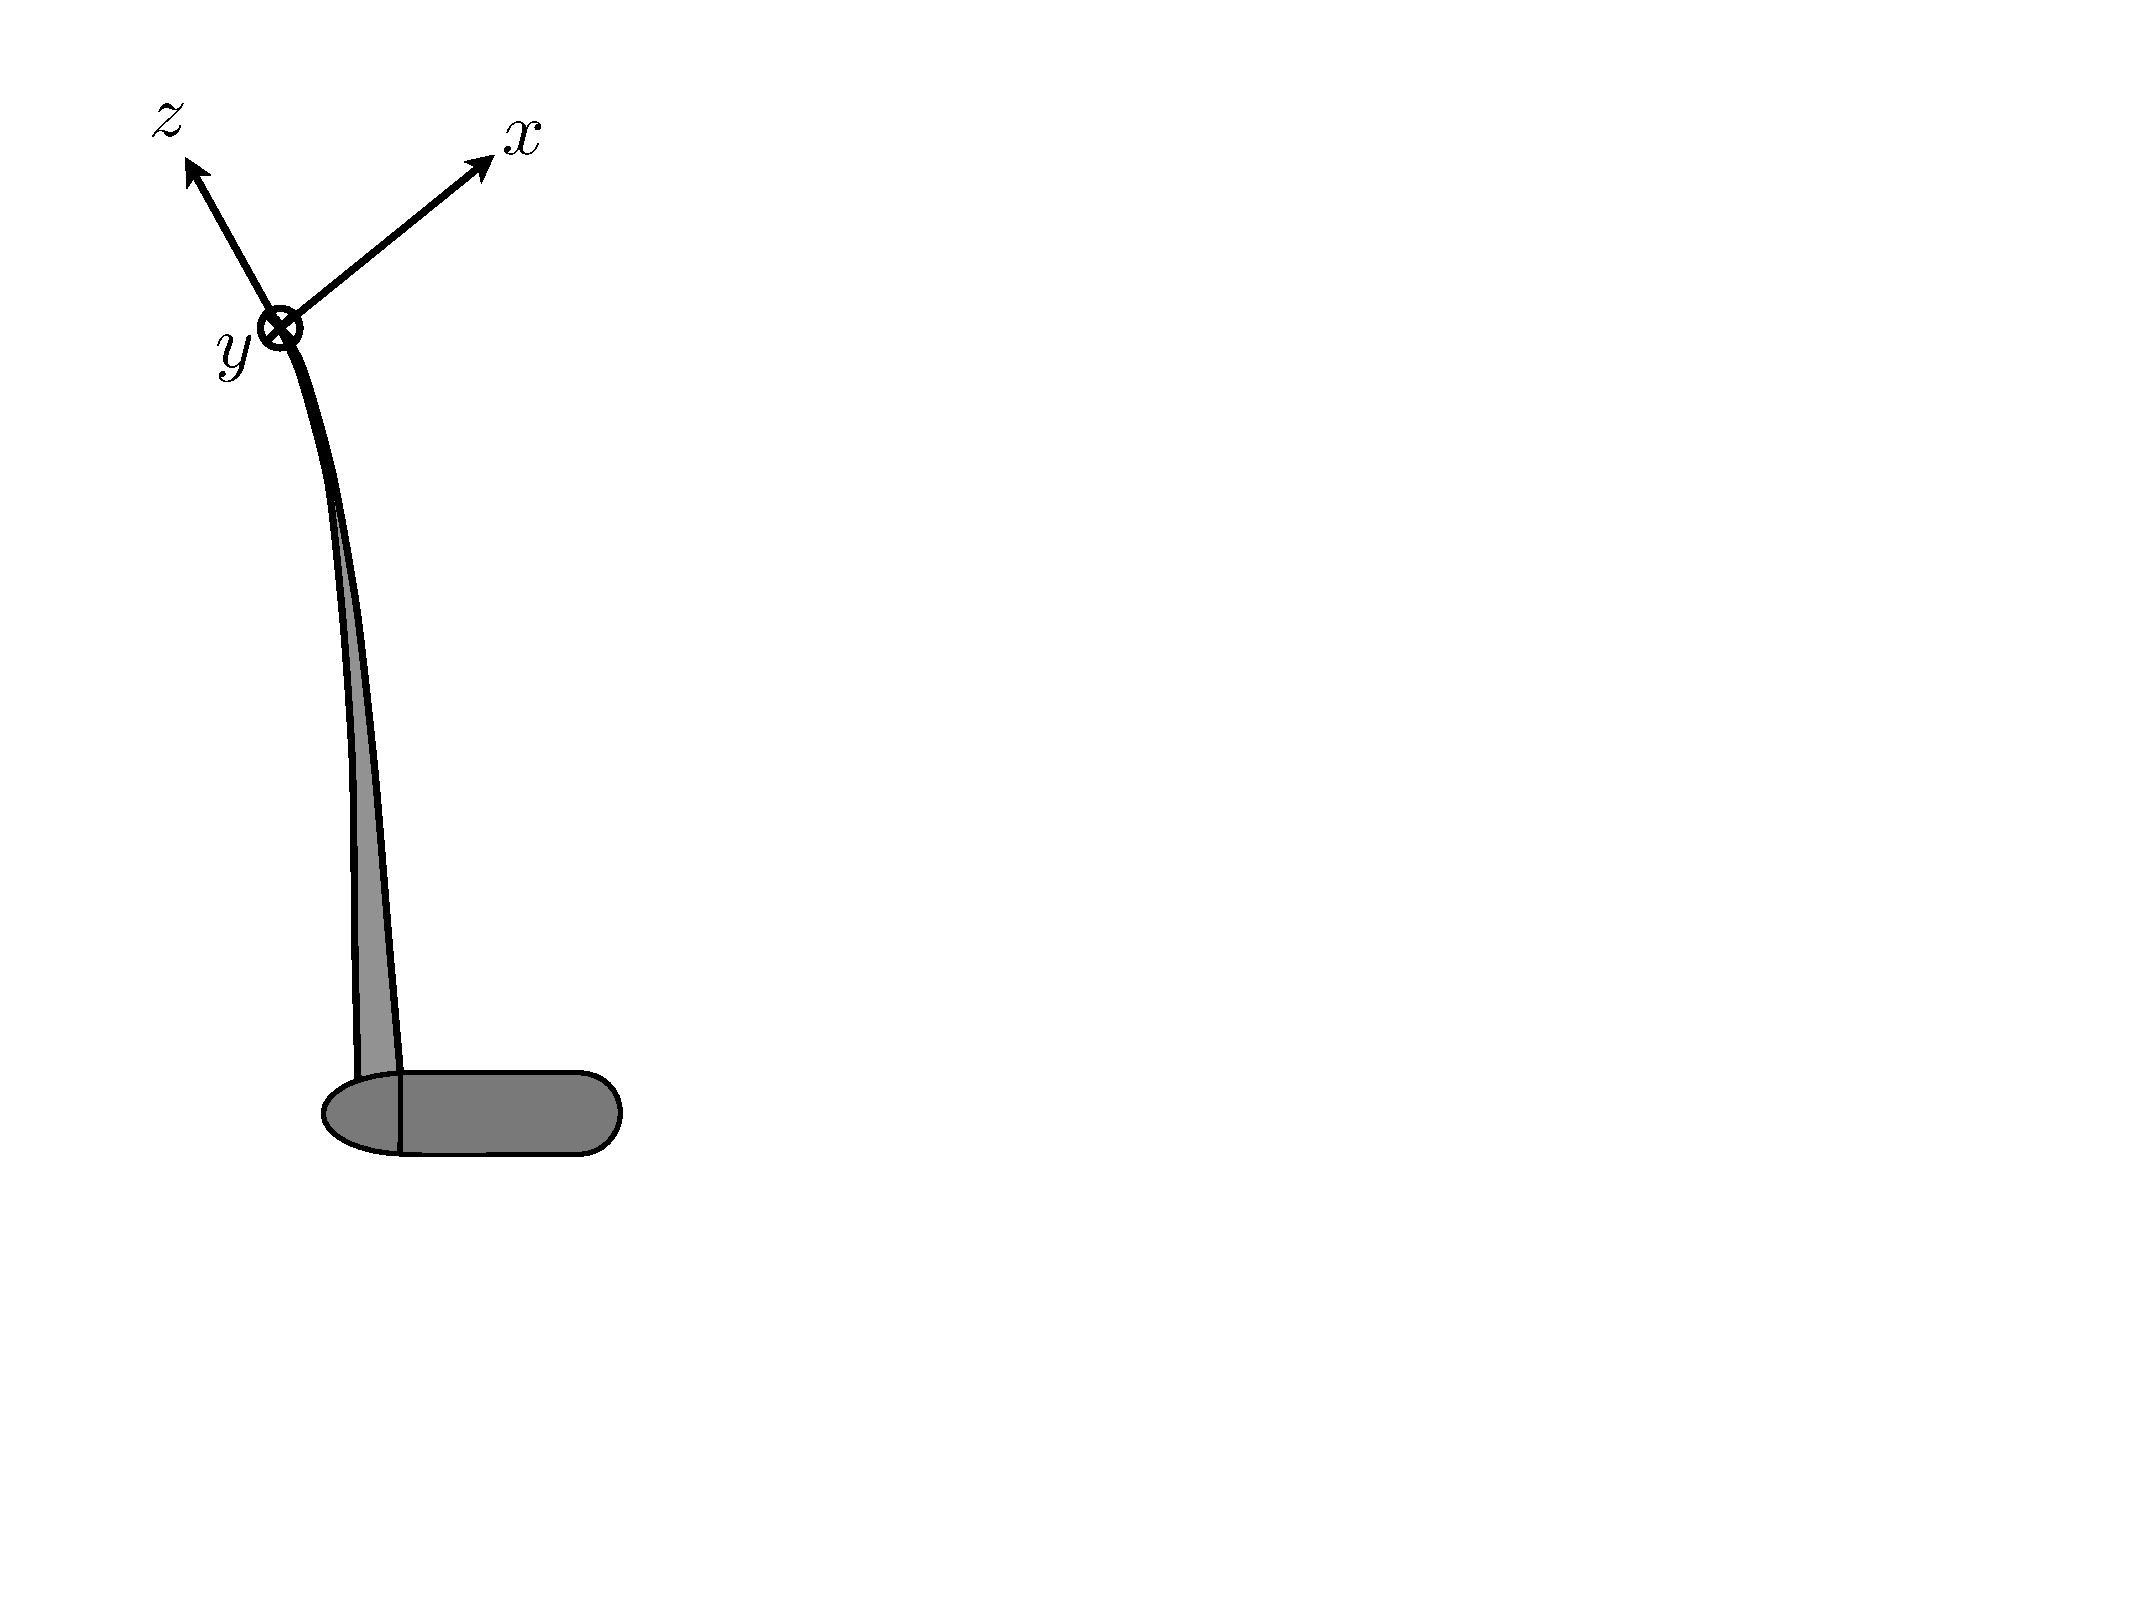
\includegraphics[height=2.5in]{figures/curved}}
   \label{fig:curved}
 }
 \qquad
 \subfloat[Front view of swept blade.  Sweep is accomplished through shearing, so coordinate system stays parallel to sweep of blade root.]{
   \makebox[3.0in][c]{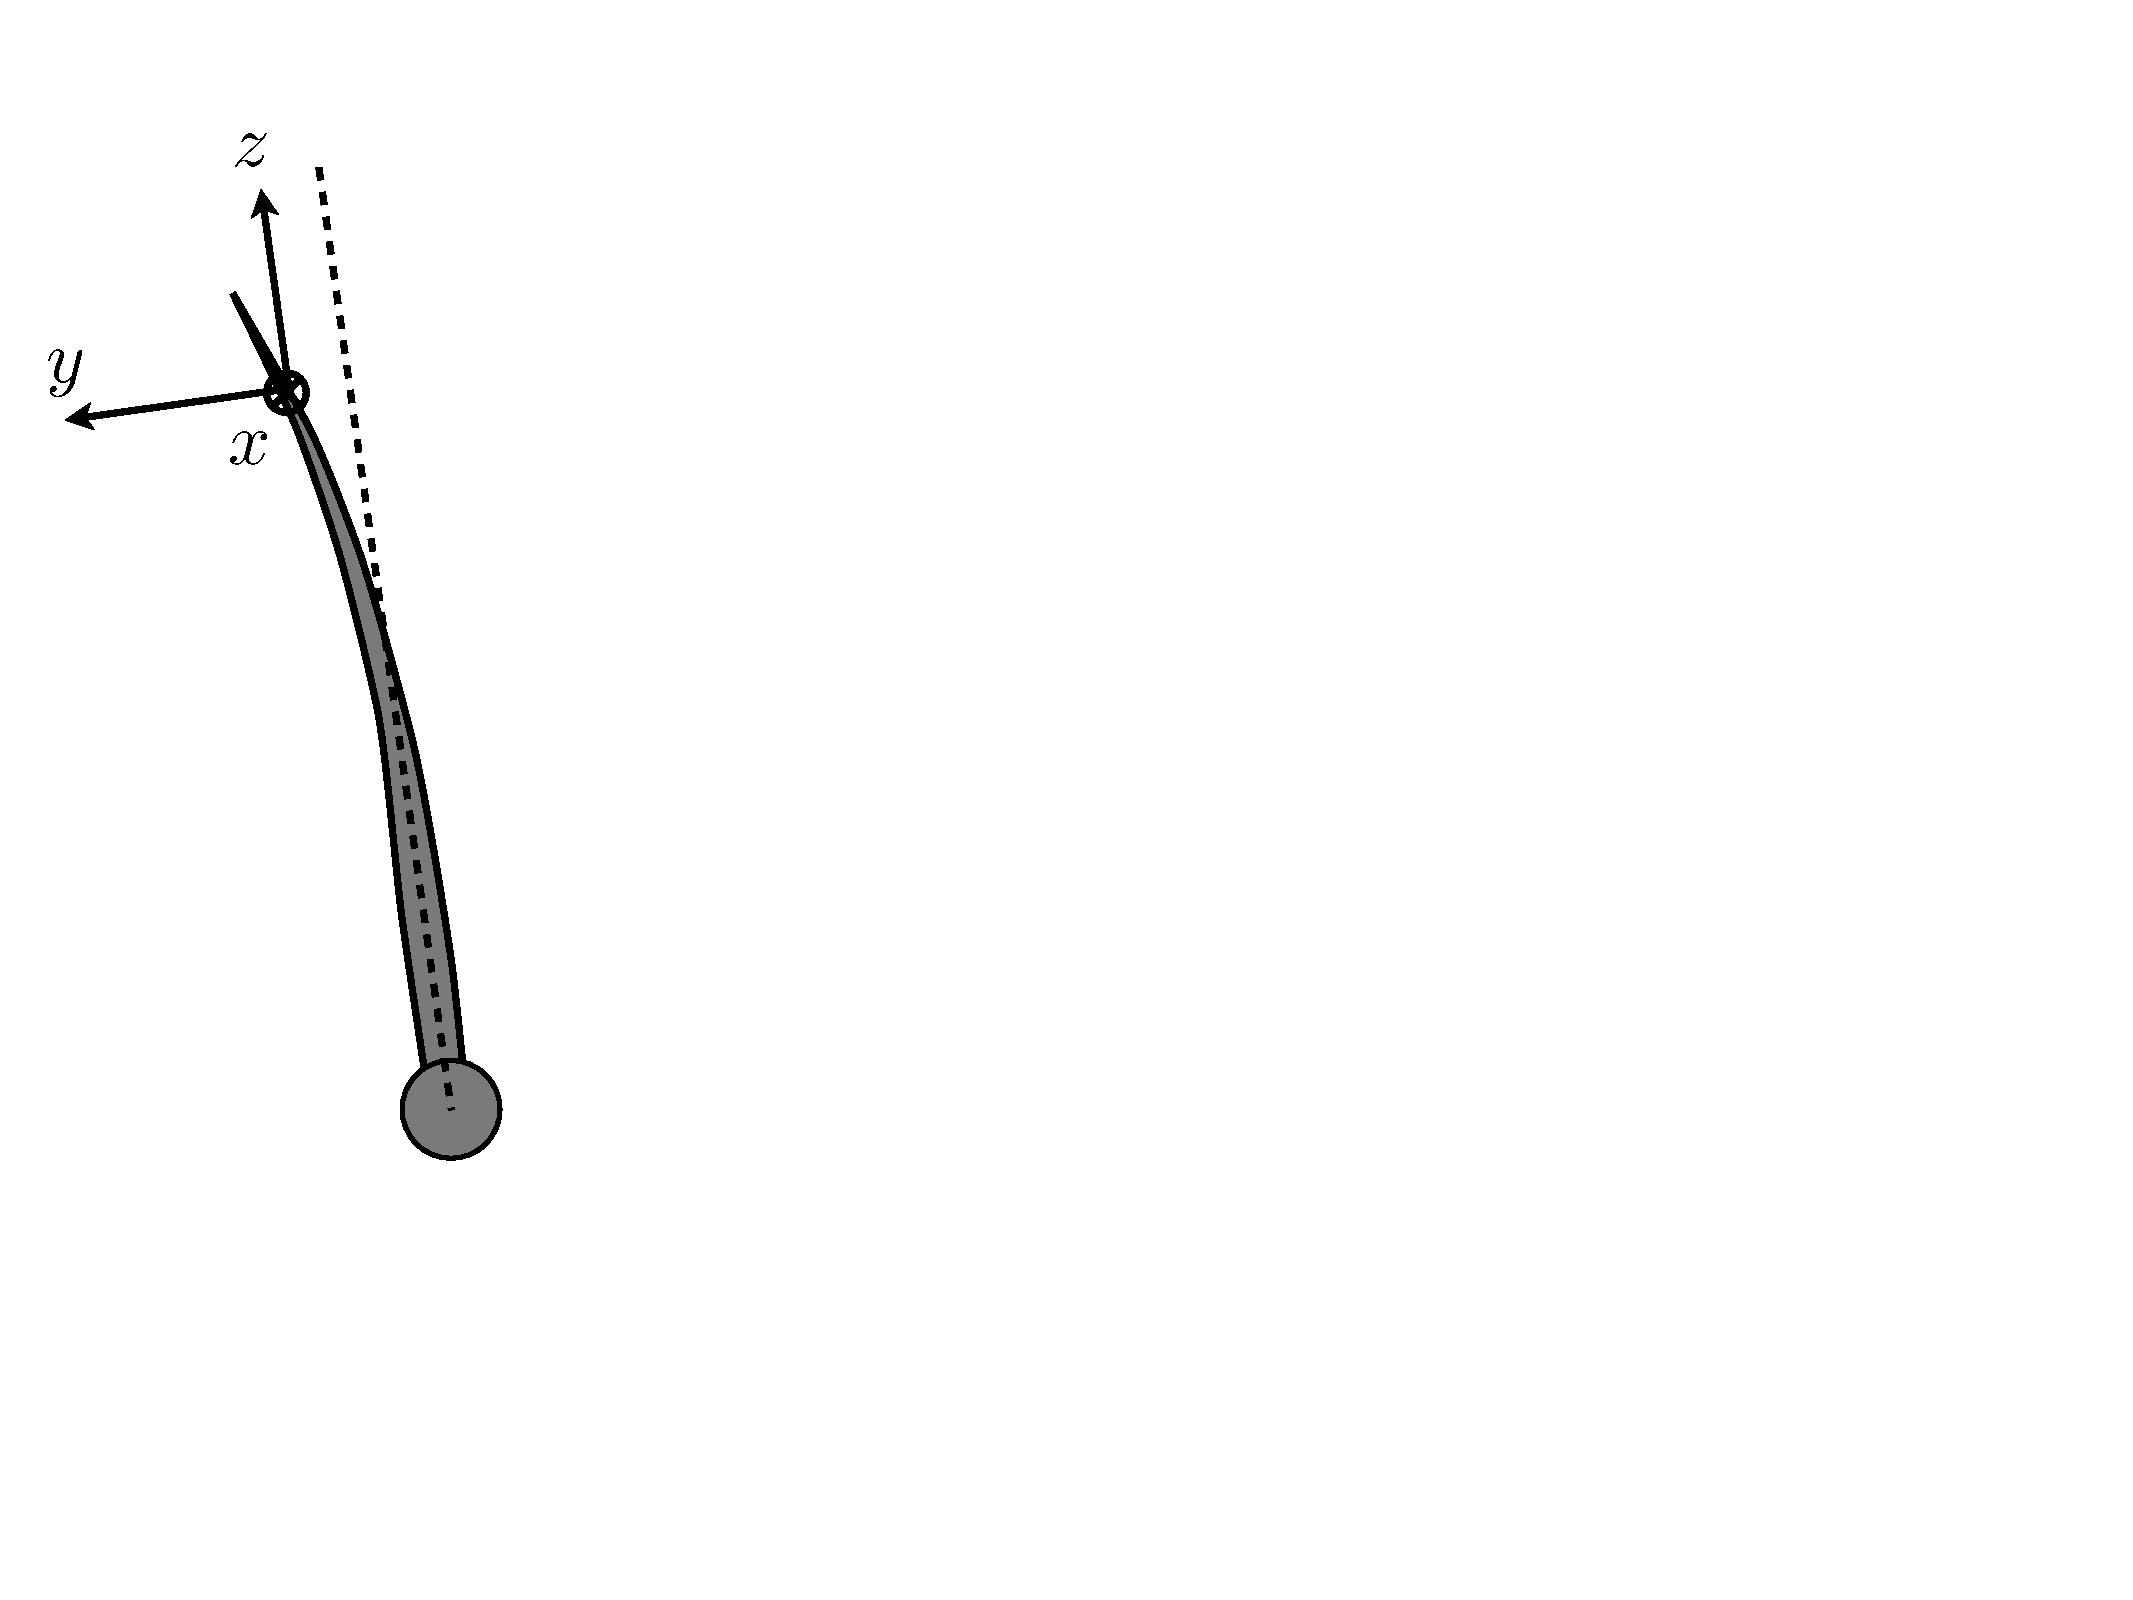
\includegraphics[height=2.5in]{figures/swept}}
   \label{fig:swept}
 }
 \caption{Definition of local airfoil coordinate system.}
 \label{fig:csys}
\end{figure}

Using this coordinate system (which is consistent with those used earlier in the paper), the normal force per unit length ($N^\prime$) is in the +x direction, and the tangential force per unit length ($T^\prime$) is in the -y direction.  If we define the precone angle as $\Phi$ then the thrust can be found through integration as:
% If we define the coning angle along the blade as $\Phi(s)$ (add figure) then the thrust can be found through integration as:
\begin{equation}
   % T = \int_0^R N^\prime \cos\Phi dr
   T_i = \int_0^R N^\prime \cos\Phi dr
\end{equation}
the torque is given by
\begin{equation}
    % Q = \int_0^R T^\prime (z \cos\phi + x\sin\phi) dr
    Q_i = \int_0^R T^\prime r \cos\Phi dr
\end{equation}

These integrals actually give the instantaneous thrust and torque and a particular azimuthal angle, and for one blade.  To get the total thrust and torque for the rotor, we need to azimuthally average and multiply by the number of blades:
\begin{equation}
\begin{aligned}
    T &= \frac{B}{2\pi}\int_0^{2\pi} T_i d\theta\\
    Q &= \frac{B}{2\pi}\int_0^{2\pi} Q_i d\theta\\
\end{aligned}
\end{equation}
Usually, this integration is done fairly coarsely by computing the instantaneous thrust and torque at a few different equally spaced azimuthal positions (e.g., 4 or 8) and then averaging those instantaneous values.  Of course, if there is no variation in inflow across the rotor, then no averaging is required.  Power is then given by
\begin{equation}
    P = \Omega Q
\end{equation}

Finally, normalization of these quantities is often desirable.  For turbines we normalize the thrust coefficient, torque coefficient, and power coefficient using:
\begin{equation}
\begin{aligned}
q &= \frac{1}{2} \rho V_{hub}^2\\
A &= \pi R_p^2\\
C_T &= \frac{T}{q A}\\
C_Q &= \frac{Q}{q R A}\\
C_P &= \frac{P}{q A V_{hub}}\\
\end{aligned}
\end{equation}
where $V_{hub}$ is the hub velocity, and $R_p$ is the projected rotor radius, or $R \cos\Phi$ using our nomenclature.  These values are normally tabulated versus the tip-speed ratio defined as:
\begin{equation}
    \lambda = \frac{\Omega R_p}{V_{hub}}
\end{equation}

For propellers, a different normalization is used, as per usual convention.  The power coefficient is generally of less interest here, as power is an input.  Instead, the efficiency is of interest, which is defined as the forward power produced relative to the power input.
\begin{equation}
\begin{aligned}
n &= \frac{\Omega}{2 \pi} \\
C_T &= \frac{T}{\rho n^2 D_p^4}\\
C_Q &= \frac{Q}{\rho n^2 D_p^5}\\
\eta &= \frac{T V_{hub}}{P} \\
% \eta &= \frac{C_T}{C_Q} \frac{J}{2 \pi} \\
\end{aligned}
\end{equation}
where $n$ is the rotation rate in revolutions/sec (instead of rad/s) and $D_p = 2 R_p$ is the projected diameter.  These quantities are normally tabulated as functions of the advance ratio (essentially the inverse of the tip-speed ratio):
\begin{equation}
    J = \frac{V_{hub}}{D_p n}
\end{equation}


\bibliographystyle{aiaa}
\bibliography{/Users/andrewning/Dropbox/BYU/References/flow}

\end{document}
